% Introdução

\documentclass[Tese.tex]{subfiles}

\begin{document}
	
\chapter{Mudança de fase}\label{ch:mudanca-de-fase}

A mudança de fase é o processo no qual um material reorganiza sua estrutura molecular ou atômica, alternando entre diferentes estados físicos, como sólido, líquido e gasoso. Em geral, esse fenômeno ocorre devido à variação de temperatura e pressão no material. Entretanto, na mudança de fase entre os estados sólido e líquido, o efeito da pressão geralmente exerce uma influência secundária, sendo a temperatura o fator principal a ser considerado.

Neste capítulo, apresentamos um modelo numérico para a mudança de fase do estado sólido para o líquido (fusão), e do líquido para o sólido (solidificação). Inicialmente, focamos em um contexto puramente térmico, desconsiderando deformações e demais efeitos mecânicos, ou seja, mantendo os pontos do domínio fixos no espaço. Esse tipo de problema tem como objetivo descrever matematicamente como a interface entre as fases sólida e líquida se move ao longo do tempo, sendo comumente conhecido como problema de Stefan. Os métodos de solução nesse caso já são bem consolidados na literatura, sendo utilizados como referências os trabalhos de \citeonline{Rolph1982}, \citeonline{Celentano1994}, \citeonline{CELENTANO1996647} e \citeonline{Bobach2021}. 

Por fim, partimos para o problema termo-mecânico da mudança de fase, onde o material pode deformar-se durante o processo. Nesta etapa, são utilizados como referência os trabalhos de \citeonline{Onate2009,Onate2010}, \citeonline{Onate2013} e \citeonline{FRANCI2017711}, embora a formulação desenvolvida no presente trabalho seja original.

\section{Formulação puramente térmica}\label{sec:mudanca-de-fase-termica}

Durante a fusão, o material absorve energia para a reestruturação das moléculas. Durante a solidificação, o material libera energia. A medida de energia que controla esses processos é denominada entalpia. Definimos a entalpia específica por unidade de volume na configuração inicial como
\begin{equation}
\enthalpy = \helmholtz + \temp\entropy + \J\p
\end{equation}
onde, conforme definido nos capítulos anteriores, $\helmholtz$ é a energia livre de Helmholtz por unidade de volume na configuração inicial, $\temp$ a temperatura absoluta, $\entropy$ a entropia por unidade de volume na configuração inicial, $\J$ o jacobiano ou deformação volumétrica, e $\p$ a pressão.

No contexto puramente térmico, $\helmholtz$ depende apenas da temperatura, e a entropia é dada por $\entropy = -\partial\helmholtz/\partial\temp$, conforme visto na \cref{eq:const2-0}. Logo, a entalpia e a sua taxa são dadas pelas expressões:
\begin{align}
&\enthalpy = \helmholtz - \temp\dfrac{\partial\helmholtz}{\partial\temp} + \J\p \\
&\dotenthalpy = \cancel{\dfrac{\partial\helmholtz}{\partial\temp}\dottemp} - \cancel{\dottemp\dfrac{\partial\helmholtz}{\partial\temp}} - \temp\dfrac{\partial^2\helmholtz}{\partial\temp^2}\dottemp + \dotJ\p + \J\dotp = - \temp\dfrac{\partial^2\helmholtz}{\partial\temp^2}\dottemp + \dotJ\p + \J\dotp. \label{eq:dotenthalpy}
\end{align}
Os termos envolvendo as taxas do Jacobiano ($\dotJ$) e da pressão ($\dotp$) são particularmente relevantes para materiais gasosos, devido às mudanças volumétricas significativas que ocorrem com variações de pressão e temperatura. No entanto, para sólidos e líquidos, onde as variações volumétricas são geralmente muito pequenas, esses termos podem ser considerados insignificantes em comparação com os demais, sendo comumente desprezados. Assim, temos:
\begin{equation}\label{eq:dotenthalpy2}
\dotenthalpy \approx - \temp\dfrac{\partial^2\helmholtz}{\partial\temp^2}\dottemp = \temp\dfrac{\partial\entropy}{\partial\temp}\dottemp = \temp\dotentropy
\end{equation}
Aplicando a \cref{eq:dotenthalpy2} na \cref{eq:cond0-0}, podemos reescrever a equação da condução de calor puramente térmica na forma
\begin{equation}\label{eq:cond0-enthalpy}
\dotenthalpy - \calorInt + \gradientei\cdot\qi = 0.
\end{equation}

Em casos onde não ocorra mudança de fase, a \cref{eq:cond0-enthalpy} deve coincidir com a \cref{eq:equacao-conducao-local-0}. Logo, teríamos $\dotenthalpy = \volumetricHeatCapacity\dottemp$, onde $\volumetricHeatCapacity$ é o calor específico volumétrico do material. Essa relação é válida tanto para sólidos quanto para fluidos. Dado que $\volumetricHeatCapacity$ é um parâmetro positivo, ela indica que variações positivas na entalpia resultam em variações positivas na temperatura, e vice-versa. Entretanto, durante o processo de mudança de fase, a relação entre entalpia e temperatura se altera, pois parte da energia é utilizada para os rearranjos moleculares, e não apenas para o aumento da temperatura.

A mudança de fase pode ser classificada como isotérmica ou não-isotérmica. Na mudança de fase isotérmica, toda a energia fornecida ou retirada do sistema é utilizada exclusivamente para a mudança de estado, não havendo variações de temperatura durante o processo. Já na mudança de fase não-isotérmica, apenas parte da energia é convertida, resultando em variações de temperatura ao longo do processo.

A quantidade de energia absorvida ou liberada (i.e. a variação de entalpia) durante a mudança de fase é denominada calor latente, denotada por $\latentHeat$. O calor latente é uma propriedade intrínseca do material. Para mudanças de fase entre sólido e líquido, onde o efeito da pressão não é significativo, ele pode ser tratado como um parâmetro fixo.

As temperaturas nas quais ocorrem as transições de fase também podem ser consideradas parâmetros fixos do material nessas condições. A mudança de fase isotérmica é caracterizada por uma única temperatura de fusão ou solidificação, denotada por $\tempm$. Quando a temperatura do material é inferior a $\tempm$, ele está na fase sólida; quando a temperatura é superior a $\tempm$, ele está na fase líquida; e quando a temperatura é exatamente igual a $\tempm$, ele está em uma fase de transição, também conhecida como fase pastosa.

Em contraste, a mudança de fase não-isotérmica é caracterizada por duas temperaturas: a temperatura limite do estado sólido, denotada por $\solidusTemp$, e a temperatura limite do estado líquido, denotada por $\liquidusTemp$. Neste caso, quando a temperatura do material é inferior a $\solidusTemp$, ele está na fase sólida; quando a temperatura é superior a $\liquidusTemp$, ele está na fase líquida; e quando a temperatura está entre $\solidusTemp$ e $\liquidusTemp$, ele está na fase de transição.

A \cref{fig:enthalpy} ilustra a relação característica entre entalpia e temperatura para os casos isotérmico e não-isotérmico, indicando as fases associadas a cada intervalo. Esses gráficos são específicos de cada material, podendo apresentar uma configuração linear por partes ou totalmente não-linear.


\begin{figure}[!htb]
	\centering
	\caption{Relações características entre entalpia e temperatura}
	\label{fig:enthalpy}
	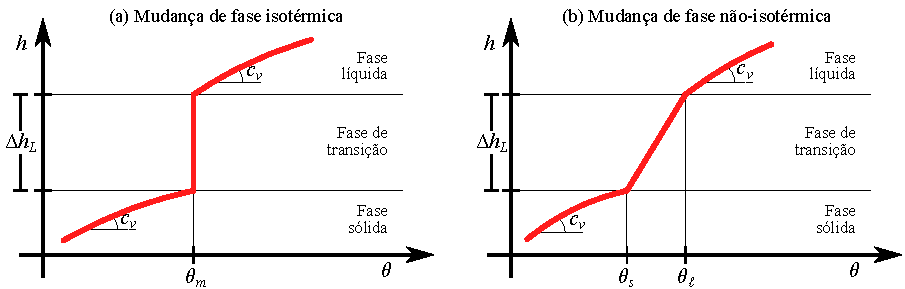
\includegraphics[scale=1.05]{Figuras/enthalpy.pdf}
	%\caption*{\textbf{Fonte:} Elaborado pelo autor}
\end{figure}

No caso isotérmico, a entalpia do sistema não pode ser unicamente determinada pela temperatura, devido à descontinuidade do gráfico durante a mudança de fase. Por esse motivo, formulações tradicionais de transferência de calor baseadas puramente em temperatura, como a apresentada no \cref{ch:termodinamica}, não são capazes de modelar esse problema de forma exata. Algumas abordagens alternativas para lidar com esse desafio são:
\begin{enumerate}[label=(\alph*)]
	\item Usar um modelo não-isotérmico aproximadamente equivalente, tomando as temperaturas limite como $\solidusTemp = \tempm - \tempvar$ e $\liquidusTemp = \tempm + \tempvar$, onde $\tempvar$ é uma variação de temperatura suficientemente pequena. É importante destacar que, além de aproximado, esse método pode apresentar instabilidades numéricas caso $\tempvar$ seja muito pequeno. Entretanto, é uma alternativa de simples implementação;\label{item:nao-isotermico}
	\item Formular as equações da termodinâmica em termos da entalpia, com base na \cref{eq:cond0-enthalpy}, tratando-a como a variável principal do sistema, ao invés da temperatura \cite{NEDJAR20029}. Essa estratégia é eficaz, pois a temperatura pode sempre ser unicamente determinada pela entalpia, enquanto a recíproca não é válida.
\end{enumerate}

Neste trabalho, focaremos apenas na mudança de fase não-isotérmica. Em casos onde for necessário modelar materiais com mudança de fase isotérmica, adotaremos a abordagem aproximada descrita no item \ref{item:nao-isotermico}.

\subsection{Modelo de mudança de fase não-isotérmica}\label{sec:mudanca-nao-isotermica}

Com base na \cref{fig:enthalpy}(b), vamos supor que a entalpia varia linearmente em relação à temperatura durante a mudança de fase. Conforme discutido anteriormente, a inclinação dessa reta possui efeito similar ao calor específico volumétrico. 

Para modelar esse comportamento, admitimos que a energia livre de Helmholtz pode ser decomposta na seguinte forma:
\begin{equation}
\helmholtz(\temp) = \helmholtzt(\temp) + \helmholtzL(\temp),
\end{equation}
onde $\helmholtzt$ é a parcela associada ao calor específico do material, que pode ser definida de forma análoga à \cref{eq:helmholtz-t-0}, e $\helmholtzL$ é uma parcela associada ao calor latente. Para representar o efeito desejado, a parcela de calor latente pode ser definida como
\begin{equation}\label{eq:helmholtzL}
\helmholtzL(\temp) = 
\begin{cases}
0 			&\text{, para }\temp \leq \solidusTemp\\[0.3cm]
\dfrac{\latentHeat}{\liquidusTemp-\solidusTemp}\left(\temp - \solidusTemp - \temp\ln\dfrac{\temp}{\solidusTemp}\right)&\text{, para }\solidusTemp < \temp < \liquidusTemp \\[0.3cm]
\latentHeat\left(1 - \temp\dfrac{\ln(\liquidusTemp/\solidusTemp)}{\liquidusTemp-\solidusTemp}\right)			&\text{, para }\temp \geq \liquidusTemp.
\end{cases}
\end{equation}
Essa energia é expressa utilizando como referência a temperatura limite do sólido ($\solidusTemp$). Destacamos, no entanto, que essa escolha é arbitrária e poderia ser feita com base em outra temperatura de referência, desde que se mantenham consistentes as derivadas necessárias para as equações subsequentes.

A partir disso, podemos definir a parcela da entropia associada ao calor latente por meio da expressão
\begin{equation}
\entropyL(\temp) = -\dfrac{\partial\helmholtzL}{\partial\temp} = 
\begin{cases}
0 			&\text{, para }\temp \leq \solidusTemp\\[0.3cm]
\latentHeat\dfrac{\ln(\temp/\solidusTemp)}{\liquidusTemp-\solidusTemp} &\text{, para }\solidusTemp < \temp < \liquidusTemp \\[0.3cm]
\latentHeat\dfrac{\ln(\liquidusTemp/\solidusTemp)}{\liquidusTemp-\solidusTemp}			&\text{, para }\temp \geq \liquidusTemp.
\end{cases}
\end{equation}
Assim, a parcela de entalpia associada ao calor latente é calculada como
\begin{equation}\label{eq:enthalpyL}
\enthalpyL(\temp) = \helmholtzL + \temp\entropyL = 
\begin{cases}
0 			&\text{, para }\temp \leq \solidusTemp\\[0.3cm]
\latentHeat\dfrac{\temp - \solidusTemp}{\liquidusTemp-\solidusTemp} &\text{, para }\solidusTemp < \temp < \liquidusTemp \\[0.3cm]
\latentHeat			&\text{, para }\temp \geq \liquidusTemp.
\end{cases}
\end{equation}
Essa definição é consistente com o modelo almejado, pois apresenta uma variação linear de entalpia entre $0$ e $\latentHeat$ ao longo da mudança de fase. Ao adicionar o efeito do calor específico, obtemos o comportamento ilustrado na \cref{fig:enthalpy}(b).

Utilizando as expressões anteriores, podemos calcular a taxa de entalpia total neste caso como
\begin{equation}\label{eq:dotenthalpy3}
\dotenthalpy = - \temp\dfrac{\partial^2\helmholtz}{\partial\temp^2}\dottemp = - \temp\left(\dfrac{\partial^2\helmholtzt}{\partial\temp^2} + \dfrac{\partial^2\helmholtzL}{\partial\temp^2}\right)\dottemp = \left(\volumetricHeatCapacity + \volumetricHeatCapacityL\right)\dottemp,
\end{equation}
onde $\volumetricHeatCapacityL$ é o calor específico volumétrico latente, definido pela expressão
\begin{equation}\label{eq:cl}
\volumetricHeatCapacityL = -\temp\dfrac{\partial^2\helmholtzL}{\partial\temp^2} = \temp\dfrac{\partial\entropyL}{\partial\temp} =
\begin{cases}
0 			&\text{, para }\temp \leq \solidusTemp\\[0.3cm]
\dfrac{\latentHeat}{\liquidusTemp-\solidusTemp} &\text{, para }\solidusTemp < \temp < \liquidusTemp \\[0.3cm]
0			&\text{, para }\temp \geq \liquidusTemp,
\end{cases}
\end{equation}
e $\volumetricHeatCapacity$ é o calor específico volumétrico do material, já apresentado nos capítulos anteriores, sendo definido neste contexto como
\begin{equation}
\volumetricHeatCapacity = -\temp\dfrac{\partial^2 \helmholtzt}{\partial \temp^2}.
\end{equation}

Vale destacar que, para representar fielmente o comportamento da \cref{fig:enthalpy}(b), o valor de $\volumetricHeatCapacity$ deveria ser nulo durante a fase de transição, uma vez que o valor de $\volumetricHeatCapacityL$ na \cref{eq:cl} já representa exatamente a inclinação do gráfico nessa fase. Alternativamente, pode-se manter a continuidade de $\volumetricHeatCapacity$, ajustando apenas o valor de $\latentHeat$ para refletir a variação de entalpia desejada. Neste trabalho, adotamos essa última abordagem.

Aplicando a \cref{eq:dotenthalpy3} na \cref{eq:cond0-enthalpy}, obtém-se, enfim, a equação da condução de calor local Lagrangiana considerando a mudança de fase não-isotérmica:
\begin{equation}\label{eq:cond-enthalpy}
\left(\volumetricHeatCapacity + \volumetricHeatCapacityL\right)\dottemp - \calorInt + \gradientei\cdot\qi = 0.
\end{equation}
Como podemos observar, o efeito do calor latente na equação de calor é similar ao efeito do calor específico, sendo a sua contribuição relevante apenas durante a mudança de fase. O termo $\volumetricHeatCapacity + \volumetricHeatCapacityL$ pode ser tratado como um calor específico volumétrico efetivo, tornando a implementação numérica quase completamente similar à apresentada na \cref{sec:mef-termo}, com a única diferença sendo a presença de descontinuidades no calor específico, dada a definição de $\volumetricHeatCapacityL$. Conforme será visto na próxima seção, essas descontinuidades podem causar instabilidades e problemas de convergência, exigindo técnicas adicionais de ajuste do modelo numérico.

\subsection{Implementação numérica}\label{sec:implementacao-mudanca-fase}

Partindo da \cref{eq:cond-enthalpy}, e aplicando os mesmos procedimentos detalhados no \cref{ch:termodinamica}, podemos construir um sistema de equações para resolver globalmente o problema térmico utilizando o método dos elementos finitos. Esse sistema seguirá a forma apresentada na \cref{eq:conducao-final}, diferenciando-se apenas na definição da matriz $\matC$, que agora deve levar em conta tanto o calor específico volumétrico ($\volumetricHeatCapacity$) quanto o calor específico latente ($\volumetricHeatCapacityL$).

A descontinuidade de $\volumetricHeatCapacityL$ introduz automaticamente uma não-linearidade ao problema, ainda que o sistema possa ser linear por partes. Para lidar com essa não-linearidade, o procedimento básico é o seguinte para cada passo de tempo: 
\begin{enumerate}
	\item Inicialmente, consideram-se as temperaturas iguais às do passo anterior. 
	\item Para cada ponto de integração do domínio, determina-se, a partir da temperatura, se o ponto está na fase sólida, líquida ou de transição;\label{itm:verifica-fase}
	\item Se o ponto estiver na fase de transição, adiciona-se a parcela $\volumetricHeatCapacityL = {\latentHeat}/{(\liquidusTemp - \solidusTemp)}$ ao calor específico volumétrico; caso contrário, $\volumetricHeatCapacityL = 0$, logo não se adiciona nada;\label{itm:adiciona-latente}
	\item Integram-se as contribuições de todos os pontos de integração, resolve-se o sistema global e atualizam-se as temperaturas;
	\item Com as temperaturas atualizadas, realiza-se novamente o procedimento descrito no item \ref{itm:verifica-fase}. Se houver mudança de fase em algum ponto, o passo de tempo deve ser recalculado, e segue-se para o item \ref{itm:adiciona-latente} e adiante. Caso não haja mudança, finaliza-se o passo de tempo.
\end{enumerate}

No entanto, esse processo iterativo pode falhar quando não houver estabilização de temperatura e fase em algum ponto do domínio, levando a repetições infinitas. Isso é especialmente crítico nos passos de tempo onde ocorre a mudança de fase.%, pois o algoritmo assume uma variação de temperatura contínua e linear entre os passos de tempo, quando na realidade ela deve ser linear por partes, pois sofre influência das duas fases (a do passo anterior e a atual).

Para exemplificar esse problema, imagine que em um determinado passo de tempo um ponto do material passa da fase sólida para a fase de transição. Na primeira tentativa, será utilizado o calor específico volumétrico da fase sólida ($\volumetricHeatCapacity$), e a temperatura calculada será maior que $\solidusTemp$, levando o ponto à fase de transição. Inicia-se, portanto, uma segunda tentativa, onde é utilizado o calor específico da fase de transição ($\volumetricHeatCapacity+\volumetricHeatCapacityL$). Como esse calor específico é maior, isso resulta em uma temperatura menor em comparação à tentativa anterior. Caso essa temperatura seja inferior a $\solidusTemp$, o ponto retorna à fase sólida, e a primeira tentativa se repetirá, causando um ciclo interminável de iterações.

Isso ocorre pois, no esquema iterativo apresentado, as variações de temperatura calculadas em cada tentativa levam em conta apenas os parâmetros da fase daquela tentativa. Mas, na realidade, a temperatura percorre as duas fases entre os passos de tempo, devendo, portanto, receber influência de ambas. Para levar esse fato em conta, podemos expressar a variação de temperatura $\Delta\temp$ como a soma das parcelas $\dtempLatent$ e $\Delta\temp-\dtempLatent$, onde $\dtempLatent$ é a variação de temperatura que ocorre dentro da fase de transição, e $\Delta\temp-\dtempLatent$ é a variação de temperatura que ocorre fora da fase de transição. Uma vez que cada uma dessas componentes está associada a um calor específico diferente, podemos calcular um calor específico volumétrico efetivo ($\volumetricHeatCapacityEffLatent$) tal que:
\begin{equation}\label{eq:heat-eff-latent}
(\volumetricHeatCapacityEffLatent)\Delta\temp = \underbrace{\left(\volumetricHeatCapacity\right)(\Delta\temp-\dtempLatent)}_\text{Fase líquida ou sólida} + \underbrace{\left(\volumetricHeatCapacity + \dfrac{\latentHeat}{\liquidusTemp-\solidusTemp} \right)\dtempLatent}_\text{Fase de transição}.
\end{equation}

Rearranjando a \cref{eq:heat-eff-latent}, obtemos a seguinte expressão para $\volumetricHeatCapacityEffLatent$:
\begin{equation}\label{eq:heat-eff}
\volumetricHeatCapacityEffLatent = \volumetricHeatCapacity + \left(\dfrac{\dtempLatent}{\Delta\temp}\right)\cdot\dfrac{\latentHeat}{\liquidusTemp-\solidusTemp}.
\end{equation}
Isto é, a parcela de calor latente é ponderada pela porcentagem da variação de temperatura que efetivamente ocorre dentro da fase de transição $\left({\dtempLatent}/{\Delta\temp}\right)$. A expressão que reflete essa porcentagem varia conforme o tipo de mudança de fase que ocorre no passo de tempo. Por exemplo, para uma mudança da fase sólida para a fase de transição, temos $\dtempLatent = \temp - \solidusTemp$. Logo, ${\dtempLatent}/{\Delta\temp} = (\temp - \solidusTemp)/(\temp-\prevtemp)$, onde $\prevtemp$ é a temperatura do ponto no passo anterior.

Para fins de generalização, a \cref{eq:heat-eff} também pode ser aplicada em passos de tempo sem mudança de fase. Nesse caso, o coeficiente ${\dtempLatent}/{\Delta\temp}$ assume o valor $1$ se o ponto estiver na fase de transição, e $0$ se estiver nas fases líquida ou sólida, refletindo a definição de $\volumetricHeatCapacityL$ dada na \cref{eq:cl}. Na \cref{tab:coeficiente-ponderador-latente}, são apresentadas as expressões de ${\dtempLatent}/{\Delta\temp}$ para cada possibilidade de variação de fase entre os passos de tempo.


\begin{table}[!htb]
	\centering
	\caption{Coeficiente de ponderação para a parcela latente do calor específico}
	\small
	\label{tab:coeficiente-ponderador-latente}
	{\def\arraystretch{1.5}
		\begin{tabular}{ll}
			\hline
			Variação de fase entre os passos de tempo & ${\dtempLatent}/{\Delta\temp}$ \\ \hline
			Sólido $\rightarrow$ Transição & $(\temp - \solidusTemp)/(\temp-\prevtemp)$ \\
			Transição $\rightarrow$ Sólido & $(\solidusTemp - \prevtemp)/(\temp-\prevtemp)$ \\ 
			Transição $\rightarrow$ Líquido & $(\liquidusTemp - \prevtemp)/(\temp-\prevtemp)$ \\ 
			Líquido $\rightarrow$ Transição & $(\temp - \liquidusTemp)/(\temp-\prevtemp)$ \\ 
			Sólido $\rightarrow$ Líquido & $(\liquidusTemp - \solidusTemp)/(\temp-\prevtemp)$ \\ 
			Líquido $\rightarrow$ Sólido & $(\solidusTemp - \liquidusTemp)/(\temp-\prevtemp)$ \\
			Sólido $\rightarrow$ Sólido & $0$ \\
			Líquido $\rightarrow$ Líquido & $0$ \\
			Transição $\rightarrow$ Transição & $1$ \\ \hline
		\end{tabular}\;
	}
	%\caption*{\textbf{Fonte:} Elaborado pelo autor}
\end{table}

Portanto, a matriz $\matC$ da \cref{eq:conducao-final} é dada por
\begin{equation}
\matC_{ij} = \int_{\domVoli}\volumetricHeatCapacityEffLatent\fforma^i\fforma^j d\voli = \int_{\domVoli}\left(\volumetricHeatCapacity + \dfrac{\dtempLatent}{\Delta\temp}\cdot\dfrac{\latentHeat}{\liquidusTemp-\solidusTemp}\right)\fforma^i\fforma^j d\voli,
\end{equation}
onde o coeficiente ${\dtempLatent}/{\Delta\temp}$ deve ser determinado caso a caso, levando em conta a mudança de fase ocorrida em cada ponto de integração do domínio. Também é importante notar que, nos casos onde há mudança de fase, a expressão de ${\dtempLatent}/{\Delta\temp}$ depende da temperatura atual, que não é conhecida durante o processo de solução. Assim, o sistema de equações \eqref{eq:conducao-final} torna-se não-linear, demandando métodos iterativos de solução, como o de Newton-Raphson. Apesar desse aumento na complexidade do algoritmo, a estratégia apresentada garante a convergência da solução sem a necessidade de modificações significativas no modelo. 

Outra alternativa para contornar o problema de convergência discutido previamente é a aplicação de técnicas de regularização, que suavizam o gráfico de entalpia por temperatura, eliminando as descontinuidades de $\volumetricHeatCapacityL$. Essa abordagem pode ser vista, por exemplo, em \citeonline{Bobach2021}. No entanto, é importante observar que essas técnicas essencialmente modificam o modelo, ainda que de forma aproximada, podendo ou não representar com precisão o comportamento real do material.



%\begin{algorithm}[!h]
%	\small
%	\LinesNumbered
%	\While{não houver mudanças de fase em nenhum ponto do domínio}{
%		\ForEach{elemento}{
%			\ForEach{ponto de integração do elemento}{	
%				\eIf{$\solidusTemp < \temp < \liquidusTemp$}{
%					$\volumetricHeatCapacityL = {\latentHeat}/{\liquidusTemp-\solidusTemp}$	
%				}	
%				{
%					$\volumetricHeatCapacityL = 0$
%				}	
%			}	
%		}
%	}	
%	\label{alg:mudanca-fase}
%\end{algorithm}

\subsection{Exemplo de verificação: solidificação de chapa ao longo de um eixo}

Para verificar numericamente o algoritmo desenvolvido, simula-se o exemplo de uma chapa retangular com as condições dispostas na \cref{fig:PhaseChange0}. Inicialmente, a chapa encontra-se na fase líquida, com temperatura de $0\,^{\circ}$C. Devido a uma temperatura prescrita constante de $-45\,^{\circ}$C na sua extremidade esquerda, a chapa solidifica-se ao longo do eixo $x_1$ conforme o tempo avança. Trata-se, portanto, de um problema essencialmente unidimensional, embora seja discretizado em um domínio bidimensional.

\begin{figure}[!htb]
	\centering
	\caption{Dados do exemplo de solidificação de chapa ao longo de um eixo}
	\label{fig:PhaseChange0}
	{\small
		\noindent\shadowbox{
			\parbox{15.3cm}{
				\setlength{\columnseprule}{1pt}
				\vspace{-0.2cm}
				{\centering\begin{center}
						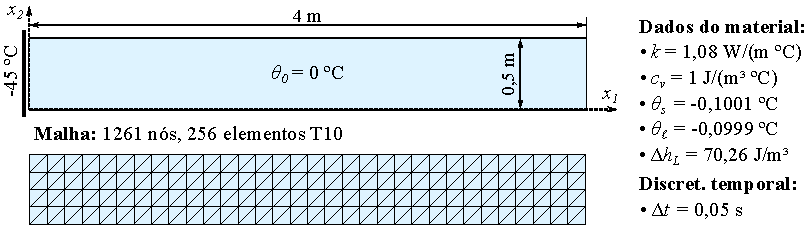
\includegraphics[scale=1.1]{Figuras/PhaseChangeExamples/PhaseChange0.pdf}
					\end{center}\par}
				\vspace{-0.2cm}
			}
		}
	}	
	%\caption*{\textbf{Fonte:} Elaborado pelo autor}
\end{figure}

Por ter sua resposta analítica conhecida, este problema é amplamente abordado na literatura como um \emph{benchmark} para modelos numéricos de mudança de fase, sendo alguns exemplos os trabalhos de \citeonline{Rolph1982} e \citeonline{Celentano1994}. Originalmente, a mudança de fase é considerada isotérmica, com temperatura de solidificação de $\tempm = -0,1\,^{\circ}$C. Neste trabalho, adaptamos o modelo para uma versão não-isotérmica aproximada, com variação de $\Delta\tempm = 10^{-4}\,^{\circ}$C, resultando nas temperaturas limites de $\solidusTemp = -0,1001\,^{\circ}$C e $\liquidusTemp = -0,0999\,^{\circ}$C.

Na \cref{fig:phaseChange0-2} são apresentados os mapas de temperatura e de fase para determinados instantes da análise, ilustrando a evolução do processo de solidificação no domínio. Na \cref{fig:phaseChange0-1}(a) é mostrada a evolução da temperatura em um ponto localizado a $1$ m da extremidade esquerda. Na \cref{fig:phaseChange0-1}(b), é apresentado o gráfico da posição da interface de mudança de fase ao longo do tempo, tomada como a coordenada $x_1$ onde a temperatura vale $-0,1\,^{\circ}$C. Os gráficos são comparados com as respostas analíticas extraídas de \citeonline{Celentano1994}, mostrando excelente concordância.

\begin{figure}[!htb]
	\centering
	\caption{Mapa de cores de temperatura e fase ao longo do tempo para o exemplo de solidificação de chapa ao longo de um eixo}
	\label{fig:phaseChange0-2}
	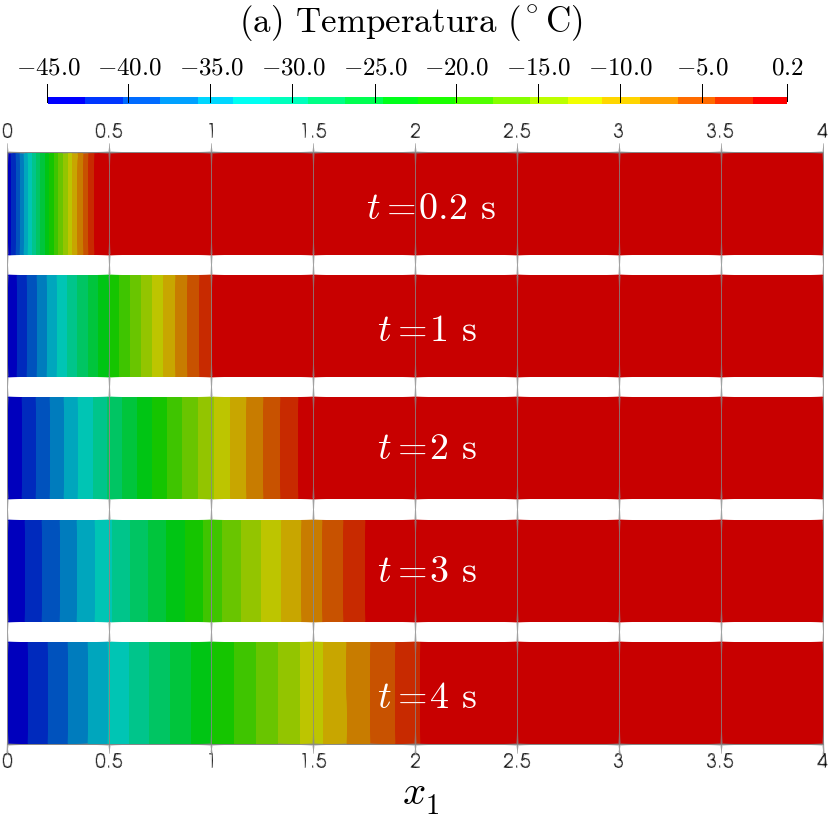
\includegraphics[scale=0.35]{Figuras/PhaseChange0/Paraview/Temperatura.png}\quad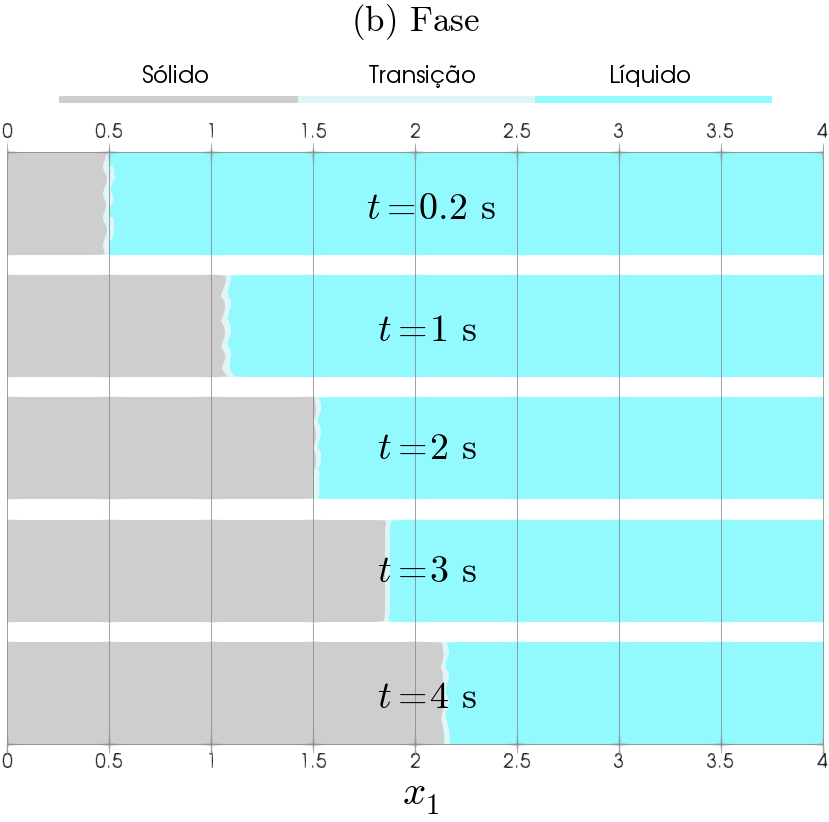
\includegraphics[scale=0.35]{Figuras/PhaseChange0/Paraview/Fase.png}
	%\caption*{\textbf{Fonte:} Elaborado pelo autor}
\end{figure}

\begin{figure}[!htb]
	\centering
	\caption{Gráficos de (a) temperatura no ponto $x_1 = 1$ m e (b) posição da interface de mudança de fase ao longo do tempo para o exemplo de solidificação de chapa ao longo de um eixo}
	\label{fig:phaseChange0-1}
	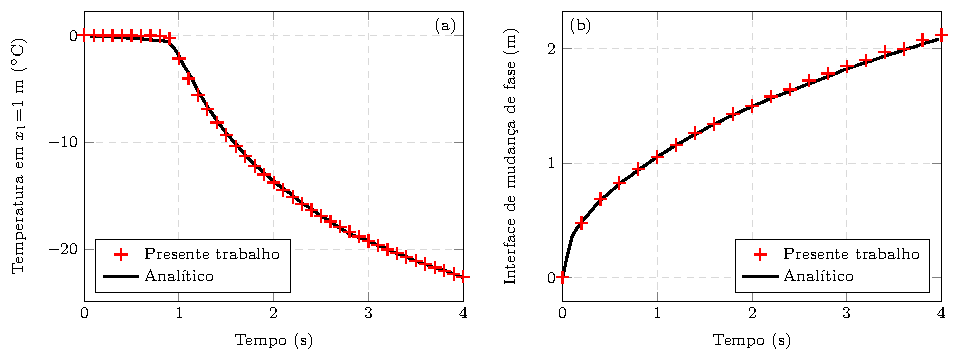
\includegraphics[scale=1]{Figuras/PhaseChange0/PhaseChange0.pdf}
	%\caption*{\textbf{Fonte:} Elaborado pelo autor}
\end{figure}

\section{Formulação termo-mecânica}\label{sec:mudanca-de-fase-termo-mecanica}

Em problemas de mudança de fase envolvendo efeitos mecânicos, deve-se levar em conta que sólidos e líquidos possuem comportamentos constitutivos diferentes, sendo necessário utilizar um modelo que leve em conta a variação de resposta mecânica ao transitar entre as fases. Neste contexto, propõe-se uma formulação Lagrangiana unificada, combinando os desenvolvimentos previamente apresentados ao longo deste trabalho.

Para a fase sólida, consideramos os modelos constitutivos discutidos nos Capítulos \ref{ch:termo-elasticidade} a \ref{ch:tvep}. Para a fase líquida, utilizamos o modelo de fluido Newtoniano apresentado na \cref{sec:incompressivelFluido}. Para a fase de transição, podemos tratar o material como um compósito, representando-o por uma combinação dos modelos de sólido e de líquido.

\subsection{Cinemática}

O uso de uma formulação totalmente Lagrangiana impõe certos desafios na definição do modelo, uma vez que a configuração indeformada do corpo varia ao longo do processo, e pode não coincidir com a configuração inicial. De fato, a configuração indeformada de um ponto no estado sólido será aquela na qual esse ponto se tornou sólido, isto é, a configuração no momento da mudança de fase. Em contrapartida, essa preocupação é menos relevante na transição da fase sólida para a líquida, pois o modelo constitutivo de fluido é baseado em grandezas Eulerianas e, portanto, sua resposta independe da configuração de referência. 

A consideração da fase de transição adiciona mais um grau de complexidade ao problema, pois, nessa fase, o domínio apresenta simultaneamente porções sólidas e líquidas, tornando necessário um modelo que leve em conta a influência de ambos os estados.

Para tratar essas particularidades, faz-se uma distinção entre as deformações ocorridas nos estados sólido e líquido. Utilizando a decomposição multiplicativa, podemos escrever a parcela mecânica do gradiente da função mudança de configuração como
\begin{equation}\label{eq:decomposicao-solido-liquida}
\Fm = \Fs\Fl,
\end{equation}
onde $\Fs$ é a parcela sólida, e $\Fl$ a parcela líquida. Dependendo do modelo de sólido adotado, $\Fs$ pode ser decomposto em parcelas mecânicas adicionais, como elásticas, viscosas e plásticas, seguindo as cinemáticas descritas nos \cref{ch:vep,ch:tvep}.

Com base em conceitos previamente discutidos sobre a decomposição multiplicativa, a forma apresentada na \cref{eq:decomposicao-solido-liquida} sugere a existência de uma configuração intermediária líquida ($\domVoll$). Como $\Fs$ é definido sobre essa configuração intermediária, esta assume o significado de configuração indeformada do sólido, garantindo a consistência do modelo independentemente da configuração inicial adotada.

A abordagem apresentada permite que as deformações sólidas e líquidas sejam tratadas individualmente. Quando o material encontra-se no estado sólido, apenas $\Fs$ é atualizado; quando o material encontra-se no estado líquido, apenas $\Fl$ é atualizado; quando o material encontra-se no estado de transição, ambos serão atualizados, e a evolução de cada componente irá depender da proporção local entre sólido e líquido, que, por sua vez, é definida em função da temperatura.

Partindo de $\Fs$ e $\Fl$, e utilizando expressões análogas às Eqs. \eqref{eq:alongamentocauchy}, \eqref{eq:E}, \eqref{eq:gradiente-velocidade}, \eqref{eq:taxa-deformacao} e \eqref{eq:mudanca-volume}, podemos definir componentes sólidas e líquidas do alongamento à direita de Cauchy-Green ($\Cs$ e $\Cl$), deformação de Green-Lagrange ($\Es$ e $\El$), velocidade da mudança de configuração ($\Ls$ e $\Ll$), taxa de deformação de engenharia ($\Ds$ e $\Dl$), e Jacobiano ($\Js$ e $\Jl$), respectivamente. 

Considerando um modelo de expansão térmica isotrópico similar ao descrito nas \cref{subsec:dec-mult-termo-elastico,sec:cinematica-tvevp}, podemos expressar o gradiente da função mudança de configuração total como
\begin{equation}
\F = \alongTermico\Fm = \alongTermico\Fs\Fl,
\end{equation}
onde $\alongTermico$ representa o alongamento térmico. As relações cinemáticas apresentadas na \cref{sec:cinematica-tvevp} também podem ser adaptadas para o presente contexto. Em particular:
\begin{align}
&\Cm = \alongTermico^{-2}\C, \label{eq:Cm}\\
&\Cs = \Fl^{-T}\Cm\Fl^{-1} = \alongTermico^{-2}\Fl^{-T}\C\Fl^{-1}, \label{eq:Cs}\\
&\dotEm = \alongTermico^{-2}\dotE - \alongTermico^{-1}\dotAlongTermico\Cm = \alongTermico^{-2}\dotE - \alongTermico^{-3}\dotAlongTermico\C, \text{\quad e} \label{eq:dotEm}\\
&\dotEs = \alongTermico^{-2}\Fl^{-T}\dotE\Fl^{-1} - \Sim(\Cs\Ll) - \alongTermico^{-1}\dotAlongTermico\Cs. \label{eq:dotEs}
\end{align}

\subsection{Base termodinâmica}

Conforme visto nos capítulos anteriores, o modelo constitutivo de um sólido possui componentes hiperelásticos, definidos através da energia livre de Helmholtz, e componentes dissipativos, cujas leis de evolução são definidas utilizando a segunda lei da termodinâmica. Por outro lado, o modelo constitutivo de fluido possui um caráter totalmente dissipativo, não armazenando energia. Reologicamente, o comportamento de um fluido pode ser representado por um pistão, similarmente ao efeito da viscosidade no sólido. 

Neste trabalho, assumimos que a fase de transição é representada reologicamente por uma associação em série entre os modelos de sólido, fluido, e de expansão térmica. Para o caso onde o sólido é um material viscoelástico-viscoplástico, por exemplo, o modelo é ilustrado na \cref{fig:phasechange-rheologic}.

\begin{figure}[!htb]
	\centering
	\caption{Modelo reológico para a fase de transição, considerando um sólido viscoelástico-viscoplástico}
	\label{fig:phasechange-rheologic}
	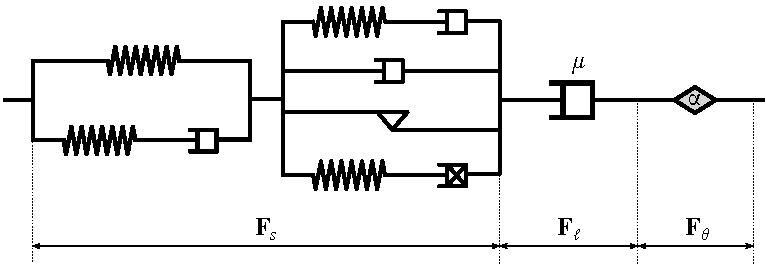
\includegraphics[scale=1]{Figuras/phasechange-rheologic.pdf}
	%\caption*{\textbf{Fonte:} Elaborado pelo autor}
\end{figure}

Generalizando o conceito discutido na \cref{subsec:dec-mult-termo-elastico}, podemos escrever a energia livre de Helmholtz do modelo como:
\begin{equation}
\helmholtz = \helmholtzt + \helmholtzL + \alongTermico^3\helmholtzm,
\end{equation}
onde $\helmholtzt$ e $\helmholtzL$ são as parcelas térmicas discutidas na \cref{sec:mudanca-nao-isotermica}, e $\helmholtzm$ representa a parcela mecânica, que pode ser adicionalmente decomposta como
\begin{equation}
\helmholtzm = \helmholtzmvol + \helmholtzmiso
\end{equation}
onde $\helmholtzmvol$ denota sua parcela volumétrica, e $\helmholtzmiso$ sua parcela isocórica. 

Assumindo que tanto o sólido quanto o fluido sejam incompressíveis, e seguindo a formulação apresentada na \cref{sec:incompressivelGeral}, temos:
\begin{equation}\label{eq:incompressivel}
\helmholtzmvol = -\p \ln(\Jm),
\end{equation}
onde $\Jm = \det\Fm$ é o Jacobiano mecânico. Embora utilizemos essa definição no presente trabalho, a formulação apresentada pode ser generalizada considerando casos compressíveis, quase-incompressíveis, ou demais modelos volumétricos.

A parcela isocórica da energia mecânica, por sua vez, deverá ser tratada individualmente em cada fase. Para a fase líquida, a componente isocórica é totalmente dissipativa, logo $\helmholtzmiso = 0$. Para a fase sólida, temos $\helmholtzmiso = \helmholtzs$, onde $\helmholtzs$ é a energia livre de Helmholtz mecânica isocórica do modelo sólido. Para a fase de transição, assumimos que $\helmholtzs$ é uma porcentagem da energia mecânica, ou seja, $\helmholtzs = \solidMultiplier\helmholtzmiso$, onde $\solidMultiplier$ é um valor entre $0$ e $1$ que depende da temperatura atual no ponto. Para garantir a continuidade da energia, $\solidMultiplier$ deve variar continuamente de $0$ a $1$ quando a temperatura varia de $\liquidusTemp$ a $\solidusTemp$. 

Com base nessas suposições, podemos estabelecer a seguinte definição:
\begin{equation}\label{eq:helmholtzmiso}
\helmholtzmiso(\temp,\Es,\internalVariables) = 
\begin{cases}
\helmholtzs(\temp,\Es,\internalVariables) 			&\text{, para }\temp \leq \solidusTemp\\
\solidMultiplier^{-1}(\temp)\helmholtzs(\temp,\Es,\internalVariables) &\text{, para }\solidusTemp < \temp < \liquidusTemp \\
0			&\text{, para }\temp \geq \liquidusTemp,
\end{cases}
\end{equation}
onde $\internalVariables$ representa, de forma geral, as variáveis internas do modelo sólido, incluindo, por exemplo, as deformações viscosas, plásticas, e as variáveis associadas aos modelos de encruamento. Assim, $\helmholtzs$ pode representar qualquer modelo de sólido dentre os discutidos nos Capítulos \ref{ch:termo-elasticidade} a \ref{ch:tvep}, apenas substituindo as deformações mecânicas totais por medidas de deformação sólidas ($\Es$ ou $\Cs$).

Considerando as variáveis independentes de cada termo apresentado, calculamos a taxa da energia livre de Helmholtz por meio da seguinte expressão:
\begin{equation}
\begin{aligned}
\dothelmholtz = &\dfrac{\partial\helmholtzt}{\partial\temp}\dottemp + \dfrac{\partial\helmholtzL}{\partial\temp}\dottemp + 3\alongTermico^2\helmholtzm\dfrac{\partial\alongTermico}{\partial\temp}\dottemp + \alongTermico^3\left(\dfrac{\partial\helmholtzmvol}{\partial\temp}\dottemp + \dfrac{\partial\helmholtzmvol}{\partial\Em}:\dotEm + \dfrac{\partial\helmholtzmvol}{\partial\p}\dotp\right) \\
& + \alongTermico^3\left(\dfrac{\partial\helmholtzmiso}{\partial\temp}\dottemp + \dfrac{\partial\helmholtzmiso}{\partial\Es}:\dotEs + \dfrac{\partial\helmholtzmiso}{\partial\internalVariables}:\dotInternalVariables\right).
\end{aligned}
\end{equation}
Aplicando as relações cinemáticas dadas nas \cref{eq:dotEm,eq:dotEs}, e manipulando algebricamente, temos:
\begin{equation}
\begin{aligned}
\dothelmholtz = &\left(\dfrac{\partial\helmholtzt}{\partial\temp} + \dfrac{\partial\helmholtzL}{\partial\temp} + 3\alongTermico^2\helmholtzm\dfrac{\partial\alongTermico}{\partial\temp} + \alongTermico^3\dfrac{\partial\helmholtzm}{\partial\temp} - \alongTermico^2\tr\mandelm\dfrac{\partial\alongTermico}{\partial\temp}\right)\dottemp  + \alongTermico^3\dfrac{\partial\helmholtzmvol}{\partial\p}\dotp\\
&+ \alongTermico\left(\dfrac{\partial\helmholtzmvol}{\partial\Em} + \Fl^{-1}\dfrac{\partial\helmholtzmiso}{\partial\Es}\Fl^{-T}\right):\dotE - \alongTermico^3\left(\Cs\dfrac{\partial\helmholtzmiso}{\partial\Es}\right):\Ll + \alongTermico^3\dfrac{\partial\helmholtzmiso}{\partial\internalVariables}:\dotInternalVariables, \label{eq:dothelmholtz-phasechange}
\end{aligned}
\end{equation}
onde $\mandelm$ é o tensor de Mandel mecânico, definido na configuração intermediária térmica, dado pela expressão
\begin{equation}
\mandelm = \Cm\dfrac{\partial\helmholtzm}{\partial\Em},
\end{equation}
que resulta em
\begin{equation}
\tr\mandelm = \Cm:\dfrac{\partial\helmholtzm}{\partial\Em} = \Cm:\dfrac{\partial\helmholtzmvol}{\partial\Em} + \Cs:\dfrac{\partial\helmholtzmiso}{\partial\Es}. \label{eq:trMm}
\end{equation}

Aplicando a \cref{eq:dothelmholtz-phasechange} na primeira lei da termodinâmica, \cref{eq:primeira-lei-2}, temos
\begin{equation}
\begin{aligned}
&-\left(\entropy+\dfrac{\partial\helmholtzt}{\partial\temp} + \dfrac{\partial\helmholtzL}{\partial\temp} + 3\alongTermico^2\helmholtzm\dfrac{\partial\alongTermico}{\partial\temp} + \alongTermico^3\dfrac{\partial\helmholtzm}{\partial\temp} - \alongTermico^2\tr\mandelm\dfrac{\partial\alongTermico}{\partial\temp}\right)\dottemp - \alongTermico^3\dfrac{\partial\helmholtzmvol}{\partial\p}\dotp\\
&+\left(\S - \alongTermico\dfrac{\partial\helmholtzmvol}{\partial\Em} - \alongTermico\Fl^{-1}\dfrac{\partial\helmholtzmiso}{\partial\Es}\Fl^{-T}\right):\dotE + \alongTermico^3\left(\Cs\dfrac{\partial\helmholtzmiso}{\partial\Es}\right):\Ll - \alongTermico^3\dfrac{\partial\helmholtzmiso}{\partial\internalVariables}:\dotInternalVariables \\
&-\temp \dotentropy + \calorInt - \gradientei\cdot\qi = 0. \label{eq:1-lei-pc}
\end{aligned}
\end{equation}
E aplicando na segunda lei da termodinâmica, \cref{eq:clausius-duhem}, temos
\begin{equation}
\begin{aligned}
\dissipation = &-\left(\entropy+\dfrac{\partial\helmholtzt}{\partial\temp} + \dfrac{\partial\helmholtzL}{\partial\temp} + 3\alongTermico^2\helmholtzm\dfrac{\partial\alongTermico}{\partial\temp} + \alongTermico^3\dfrac{\partial\helmholtzm}{\partial\temp} - \alongTermico^2\tr\mandelm\dfrac{\partial\alongTermico}{\partial\temp}\right)\dottemp - \alongTermico^3\dfrac{\partial\helmholtzmvol}{\partial\p}\dotp\\
&+\left(\S - \alongTermico\dfrac{\partial\helmholtzmvol}{\partial\Em} - \alongTermico\Fl^{-1}\dfrac{\partial\helmholtzmiso}{\partial\Es}\Fl^{-T}\right):\dotE + \alongTermico^3\left(\Cs\dfrac{\partial\helmholtzmiso}{\partial\Es}\right):\Ll - \alongTermico^3\dfrac{\partial\helmholtzmiso}{\partial\internalVariables}:\dotInternalVariables \\
& - \dfrac{1}{T}\qi\cdot\gradientei\,\temp \geq 0. \label[ineq]{eq:2-lei-pc}
\end{aligned}
\end{equation}
Utilizando essas expressões como base, derivam-se as relações constitutivas do material. O procedimento adotado varia conforme a fase, sendo detalhado individualmente para cada caso nas seções seguintes.

\subsection{Modelo constitutivo da fase sólida}\label{sec:solido}

Na fase sólida ($\temp \leq \solidusTemp$), temos $\helmholtzmiso = \helmholtzs$, e consideramos que a variação de deformação líquida é nula, ou seja, $\Ll = \mathbf{0}$. Assim, a \cref{eq:1-lei-pc} resulta em
\begin{equation}
\begin{aligned}
&-\left(\entropy+\dfrac{\partial\helmholtzt}{\partial\temp} + \dfrac{\partial\helmholtzL}{\partial\temp} + 3\alongTermico^2\helmholtzm\dfrac{\partial\alongTermico}{\partial\temp} + \alongTermico^3\dfrac{\partial\helmholtzm}{\partial\temp} - \alongTermico^2\tr\mandelm\dfrac{\partial\alongTermico}{\partial\temp}\right)\dottemp - \alongTermico^3\dfrac{\partial\helmholtzmvol}{\partial\p}\dotp\\
&+\left(\S - \alongTermico\dfrac{\partial\helmholtzmvol}{\partial\Em} - \alongTermico\Fl^{-1}\dfrac{\partial\helmholtzs}{\partial\Es}\Fl^{-T}\right):\dotE - \alongTermico^3\dfrac{\partial\helmholtzs}{\partial\internalVariables}:\dotInternalVariables -\temp \dotentropy + \calorInt - \gradientei\cdot\qi = 0, \label{eq:1-lei-pc-solido}
\end{aligned}
\end{equation}
e a \cref{eq:2-lei-pc} resulta em
\begin{equation}
\begin{aligned}
\dissipation = &-\left(\entropy+\dfrac{\partial\helmholtzt}{\partial\temp} + \dfrac{\partial\helmholtzL}{\partial\temp} + 3\alongTermico^2\helmholtzm\dfrac{\partial\alongTermico}{\partial\temp} + \alongTermico^3\dfrac{\partial\helmholtzm}{\partial\temp} - \alongTermico^2\tr\mandelm\dfrac{\partial\alongTermico}{\partial\temp}\right)\dottemp - \alongTermico^3\dfrac{\partial\helmholtzmvol}{\partial\p}\dotp\\
&+\left(\S - \alongTermico\dfrac{\partial\helmholtzmvol}{\partial\Em} - \alongTermico\Fl^{-1}\dfrac{\partial\helmholtzs}{\partial\Es}\Fl^{-T}\right):\dotE - \alongTermico^3\dfrac{\partial\helmholtzs}{\partial\internalVariables}:\dotInternalVariables - \dfrac{1}{T}\qi\cdot\gradientei\,\temp \geq 0. \label[ineq]{eq:2-lei-pc-solido}
\end{aligned}
\end{equation}

Seguindo o procedimento de \citeonline{Coleman1963}, as expressões acima devem ser válidas para qualquer processo termodinâmico, ou seja, para quaisquer valores das taxas $\dottemp$, $\dotE$ e $\dotp$. Essa condição é atendida se os conjugados termodinâmicos dessas taxas forem nulos, o que resulta nas seguintes relações constitutivas:
\begin{align}
&\entropy = - \dfrac{\partial\helmholtzt}{\partial\temp} - \dfrac{\partial\helmholtzL}{\partial\temp} - \alongTermico^3\dfrac{\partial\helmholtzm}{\partial\temp} +  \alongTermico^2\left(\tr\mandelm - 3\helmholtzm\right)\dfrac{\partial\alongTermico}{\partial\temp}, \label{eq:entropy-solid} \\[0.15cm]
&\S = \alongTermico\dfrac{\partial\helmholtzmvol}{\partial\Em} + \alongTermico\Fl^{-1}\dfrac{\partial\helmholtzs}{\partial\Es}\Fl^{-T}, \text{\quad e} \label{eq:S-solid} \\[0.15cm]
&\dfrac{\partial\helmholtzmvol}{\partial\p} = 0, \label{eq:incompress-pc}
\end{align}
onde a última é a condição de incompressibilidade, abordada no \cref{ch:materiaisIncompressiveis}. O termo ${\partial\helmholtzs}/{\partial\Es}$ representa a tensão isocórica do modelo sólido isolado, definida, neste caso, na configuração intermediária líquida. Em particular, quando não há deformações líquidas (i.e. $\Fl=\I$), a \cref{eq:S-solid} recai exatamente na tensão dos modelos sólidos discutidos em capítulos anteriores.

Relacionando as \cref{eq:trMm,eq:S-solid}, verificamos que $\tr\mandelm = \alongTermico^{-3}\C:\S$. Logo, podemos reescrever a equação da entropia como
\begin{equation}
\entropy = - \dfrac{\partial\helmholtzt}{\partial\temp} - \dfrac{\partial\helmholtzL}{\partial\temp} - \alongTermico^3\dfrac{\partial\helmholtzm}{\partial\temp} +  \left(\alongTermico^{-1}\C:\S - 3\alongTermico^2\helmholtzm\right)\dfrac{\partial\alongTermico}{\partial\temp}, \label{eq:entropy-solid-2}
\end{equation}
que é análoga à \cref{eq:entropy-vevp-2}, aplicada no caso puramente sólido, com exceção do termo de calor latente. As leis de evolução das variáveis internas também devem seguir exatamente as mesmas expressões do caso puramente sólido.

Aplicando as \cref{eq:S-solid,eq:incompress-pc,eq:entropy-solid-2} na \cref{eq:1-lei-pc-solido} e na \cref{eq:2-lei-pc-solido}, podemos reescrever a primeira e segunda leis da termodinâmica por expressões análogas às já apresentadas em capítulos anteriores:
\begin{align} 
&\temp \dotentropy + \gradientei\cdot\qi = \dissipationmec + \calorInt, \text{\quad e}\label{eq:primeira-lei-solid} \\
&\dissipation = \dissipationmec - \dfrac{1}{T}\qi\cdot\gradientei\,\temp \geq 0,  \label[ineq]{eq:clausius-duhem-solid}
\end{align}
onde a taxa de dissipação mecânica ($\dissipationmec$) na fase sólida provém apenas das variáveis internas, sendo definida de forma genérica como
\begin{equation} \label{eq:dissipation-solido}
\dissipationmec = -\alongTermico^3\left(\dfrac{\partial\helmholtzs}{\partial\internalVariables}:\dotInternalVariables\right).
\end{equation}
Para sólidos hiperelásticos, a equação acima é nula. Para sólidos com modelo viscoelástico-viscoplástico, esta é equivalente à forma já apresentada na \cref{eq:dissipation-mec}.

A implementação numérica do modelo segue uma abordagem totalmente similar ao caso puramente sólido. Para garantir a convergência quadrática da solução não-linear, calculamos o operador tangente consistente ($\CC$) através da derivada da \cref{eq:S-solid} com relação a $\E$. Considerando que $\Fl$ é constante na fase sólida, e utilizando a relação cinemática \eqref{eq:Cm}, temos
\begin{equation}\label{eq:CC-solido}
\CC = \alongTermico^{-1}\CCvol + \alongTermico^{-1}\Fl^{-1}\left(\CCs:\dfrac{\partial\Es}{\partial\Em}\right)\Fl^{-T},
\end{equation}
onde $\CCvol$ e $\CCs$ são definidos, respectivamente, como
\begin{equation}
\CCvol = \dfrac{\partial^2\helmholtzmvol}{\partial\Em\otimes\partial\Em} \text{\qquad e\qquad} \CCs = \dfrac{\partial^2\helmholtzs}{\partial\Es\otimes\partial\Es}, \label{eq:CCaux-solido}
\end{equation}
e $\partial\Es/\partial\Em$ pode ser calculado com base na \cref{eq:Cs}:
\begin{equation}
\dfrac{\partial(\Esind)_{ij}}{\partial(\Emind)_{kl}} = \dfrac{\partial(\Csind)_{ij}}{\partial(\Cmind)_{kl}} = (\Flind)^{-1}_{ki}(\Flind)^{-1}_{lj}. \label{eq:dEs_dEm}
\end{equation}
Para o modelo incompressível apresentado na \cref{eq:incompressivel}, as parcelas volumétricas da tensão e do operador tangente consistente resultam, respectivamente, em
\begin{equation}
\dfrac{\partial\helmholtzmvol}{\partial\Em} = -\p\Cm^{-1} \text{\qquad e\qquad} \CCvol =  -2\p\dfrac{\partial\Cm^{-1}}{\partial\Cm}.
\end{equation}

No \autoref{quadro:solido}, apresenta-se um resumo esquemático do modelo discutido nesta seção.

\begin{quadro}[!htb]
	\centering
	\caption{Resumo esquemático do modelo constitutivo mecânico para a fase sólida ($\temp \leq \solidusTemp$)}
	\label{quadro:solido}
	\fbox{%
		\begin{minipage}{\textwidth}
			\vspace{0.4cm}
			
			\begin{enumerate}[label=\arabic*.]
				\item \textbf{Dados:} $\temp$, $\F$, $\Fl\indprev$, $\internalVariables\indprev$.
				\item A partir de $\temp$, calcula-se $\alongTermico$ utilizando o modelo de expansão térmica. Disto, temos: 
				
				$\Fm = \alongTermico^{-1}\F \quad\rightarrow\quad \Cm = \Fm^T\Fm \quad\rightarrow\quad \Em = \frac{1}{2}(\Cm-\I)$.					
				\item Toma-se $\Fl = \Fl\indprev$, e calcula-se $\Fs = \Fm\Fl^{-1}$. Disto, temos: 
				
				$\Cs = \Fs^T\Fs \quad\rightarrow\quad \Es = \frac{1}{2}(\Cs-\I)$.
				\item Atualizam-se as variáveis internas do sólido ($\internalVariables$), caso existam, por meio das suas respectivas leis de evolução.
				\item A partir de $\Cs$ e/ou $\Es$, calcula-se ${\partial\helmholtzs}/{\partial\Es}$ utilizando o modelo de sólido.
				\item A partir de $\Cm$ e/ou $\Em$, calcula-se ${\partial\helmholtzmvol}/{\partial\Em}$ utilizando o modelo volumétrico. Caso o modelo seja incompressível, deve-se aplicar ainda a condição de incompressibilidade.
				\item Calcula-se a tensão $\S$ por meio da \cref{eq:S-solid} e o operador tangente consistente $\CC$ por meio da \cref{eq:CC-solido}.
			\end{enumerate}
		
			\vspace{0.01cm}
		\end{minipage}
	}
\end{quadro}

\subsection{Modelo constitutivo da fase líquida}\label{sec:liquido}

Na fase líquida ($\temp \geq \liquidusTemp$), a parcela $\helmholtzmiso$ é nula, bem como todas as suas derivadas. Além disso, não há variação nas deformações sólidas e nas suas variáveis internas, isto é, $\dotFs = \dotInternalVariables = \mathbf{0}$. Assim, a \cref{eq:1-lei-pc} resulta em
\begin{equation}
\begin{aligned}
&-\left(\entropy+\dfrac{\partial\helmholtzt}{\partial\temp} + \dfrac{\partial\helmholtzL}{\partial\temp} + 3\alongTermico^2\helmholtzmvol\dfrac{\partial\alongTermico}{\partial\temp} + \alongTermico^3\dfrac{\partial\helmholtzmvol}{\partial\temp} - \alongTermico^2\tr\mandelm\dfrac{\partial\alongTermico}{\partial\temp}\right)\dottemp \\
&- \alongTermico^3\dfrac{\partial\helmholtzmvol}{\partial\p}\dotp+\Siso:\dotE - \temp \dotentropy + \calorInt - \gradientei\cdot\qi = 0, \label{eq:1-lei-liquid}
\end{aligned}
\end{equation}
e a \cref{eq:2-lei-pc} resulta em
\begin{equation}
\begin{aligned}
\dissipation = &-\left(\entropy+\dfrac{\partial\helmholtzt}{\partial\temp} + \dfrac{\partial\helmholtzL}{\partial\temp} + 3\alongTermico^2\helmholtzmvol\dfrac{\partial\alongTermico}{\partial\temp} + \alongTermico^3\dfrac{\partial\helmholtzmvol}{\partial\temp} - \alongTermico^2\tr\mandelm\dfrac{\partial\alongTermico}{\partial\temp}\right)\dottemp \\
&- \alongTermico^3\dfrac{\partial\helmholtzmvol}{\partial\p}\dotp+\Siso:\dotE - \dfrac{1}{T}\qi\cdot\gradientei\,\temp \geq 0, \label{eq:2-lei-liquid}
\end{aligned}
\end{equation}
onde $\Siso$ é a parcela isocórica da tensão de Piola-Kirchhoff de segunda espécie, definida como
\begin{equation}
\Siso = \S - \alongTermico\dfrac{\partial\helmholtzmvol}{\partial\Em}.
\end{equation}

Pelo procedimento de Coleman-Noll, a condição $\Siso = \mathbf{0}$ seria capaz de atender as leis da termodinâmica. No entanto, essa solução trivial não representa o comportamento viscoso do fluido. Para garantir o caráter dissipativo do sistema, adotaremos um modelo que permita valores positivos de $\Siso:\dotE$, ainda respeitando as leis da termodinâmica.

Dado que $\dotEs = \mathbf{0}$, podemos reescrever a \cref{eq:dotEs} como
\begin{equation}
\dotE = \alongTermico^2\Fl^T\Sim\left(\Cs\Ll\right)\Fl + \alongTermico\dotAlongTermico\Cm.
\end{equation}
Utilizando a relação acima, e realizando determinadas manipulações algébricas, obtemos:
\begin{equation}\label{eq:SE-liquid}
\Siso:\dotE = \alongTermico^2\left(\Cs\Fl\Siso\Fl^T\right):\Ll + \alongTermico\dotAlongTermico\Cm:\Siso.
\end{equation}
O tensor $\Cs\Fl\Siso\Fl^T$ representa uma componente da tensão de Mandel na configuração intermediária líquida. Para materiais isotrópicos, é possível demonstrar que ele é simétrico, logo
\begin{equation}
\alongTermico^2\left(\Cs\Fl\Siso\Fl^T\right):\Ll = \alongTermico^2\left(\Cs\Fl\Siso\Fl^T\right):\Sim(\Ll) = \alongTermico^2\left(\Cs\Fl\Siso\Fl^T\right):\Dl.
\end{equation}
Esse termo representa a taxa de dissipação devida às deformações viscosas do líquido, definida por unidade de volume na configuração inicial. Para expressa-la por unidade de volume na configuração intermediária líquida, dividimos por $\Jt\Jl = \alongTermico^3\Jl$, o que resulta em  $\alongTermico^{-1}\Jl^{-1}\left(\Cs\Fl\Siso\Fl^T\right):\Dl$. Logo, $\alongTermico^{-1}\Jl^{-1}\Cs\Fl\Siso\Fl^T$ é conjugado termodinâmico de $\Dl$. Para garantir a não-negatividade da dissipação, podemos adotar uma relação linear entre esses termos. Em particular, para um fluido Newtoniano, adotamos:
\begin{equation}\label{eq:visc-liquido}
2\viscfluid\Dl = \alongTermico^{-1}\Jl^{-1}\Cs\Fl\Siso\Fl^T,
\end{equation}
onde $\viscfluid$ é o parâmetro de viscosidade do líquido. Nota-se que, ao formular o modelo com base na configuração intermediária líquida, garantimos que a resposta seja independente da configuração inicial, mantendo a consistência da formulação.

Sabendo que $\dotEl = \Fl^T\Dl\Fl$, podemos rearranjar a \cref{eq:visc-liquido} na seguinte lei constitutiva:
\begin{equation}\label{eq:lei-liquido}
\Siso = 2\viscfluid\alongTermico\Jl\Cm^{-1}\dotEl\Cl^{-1},
\end{equation}
o que resulta em 
\begin{equation}\label{eq:lei-liquido-S}
\S = \alongTermico\dfrac{\partial\helmholtzmvol}{\partial\Em} + 2\viscfluid\alongTermico\Jl\Cm^{-1}\dotEl\Cl^{-1}.
\end{equation}
Essa equação é uma generalização do modelo de fluido Newtoniano incompressível apresentado na \cref{sec:incompressivelFluido}. Nos casos onde não há deformações sólidas ou térmicas, temos $\Cm=\Cl=\C$, $\dotEl = \dotE$, $\Jl=J$ e $\alongTermico=1$, fazendo com que a \cref{eq:lei-liquido} recaia na \cref{eq:newtonianFluid1}.

O último termo da \cref{eq:SE-liquid} contribui para o conjugado termodinâmico de $\dottemp$ nas \cref{eq:1-lei-liquid,eq:2-lei-liquid}. Igualando esse conjugado a zero, e manipulando algebricamente, podemos obter a seguinte expressão para a entropia:
\begin{equation}
\entropy = - \dfrac{\partial\helmholtzt}{\partial\temp} - \dfrac{\partial\helmholtzL}{\partial\temp} - \alongTermico^3\dfrac{\partial\helmholtzmvol}{\partial\temp} +  \left(\alongTermico^{-1}\C:\S - 3\alongTermico^2\helmholtzmvol\right)\dfrac{\partial\alongTermico}{\partial\temp}, \label{eq:entropy-liquid}
\end{equation}
que é similar à \cref{eq:entropy-solid-2} da fase sólida, considerando $\helmholtzm = \helmholtzmvol$. A condição de incompressibilidade, dada na \cref{eq:incompress-pc}, mantêm-se válida no presente contexto.

Aplicando essas relações constitutivas na \cref{eq:1-lei-liquid} e na \cref{eq:2-lei-liquid}, obtemos novamente as expressões dadas na \cref{eq:primeira-lei-solid} e na \cref{eq:clausius-duhem-solid} para as leis da termodinâmica, sendo a taxa de dissipação mecânica, neste caso, definida como
\begin{equation} \label{eq:dissipation-liquid}
\dissipationmec = \alongTermico^2\left(\Cs\Fl\Siso\Fl^T\right):\Dl = 2\viscfluid\alongTermico^3\Jl\|\Dl\|.
\end{equation}

A partir das relações cinemáticas das \cref{eq:Cm,eq:dotEm}, temos ${\partial\Em}/{\partial\E} = \alongTermico^{-2}\II$, ${\partial\dotEm}/{\partial\dotE} = \alongTermico^{-2}\II$ e ${\partial\dotEm}/{\partial\E} = -2\alongTermico^{-3}\dotAlongTermico\II$. Utilizando essas relações, podemos calcular o operador tangente consistente e o operador de viscosidade do modelo na fase líquida, respectivamente, como
\begin{align}
&\CC = \dfrac{\partial\S}{\partial\Em}:\dfrac{\partial\Em}{\partial\E} + \dfrac{\partial\S}{\partial\dotEm}:\dfrac{\partial\dotEm}{\partial\E} = \alongTermico^{-1}\CCm - 2\alongTermico^{-2}\dotAlongTermico\viscOperatorm \label{eq:CC-liquido} \\[0.1cm]
&\viscOperator = \dfrac{\partial\S}{\partial\dotEm}:\dfrac{\partial\dotEm}{\partial\dotE} = \alongTermico^{-1}\viscOperatorm \label{eq:viscop-liquido}
\end{align}
onde $\CCm$ e $\viscOperatorm$ são os operadores tangente consistente e de viscosidade do modelo de fluido puramente mecânico, que podem ser calculados por expressões análogas às da \cref{sec:incompressivelFluido}. Levando em conta que $\dotAlongTermico = (\partial\alongTermico/\partial\temp)\dottemp \approx \coefExp\dottemp$, o último termo da \cref{eq:CC-liquido} pode ser desprezado para materiais com coeficiente de expansão térmica $\coefExp$ muito pequeno.

No \autoref{quadro:liquido}, apresenta-se um resumo esquemático do modelo discutido nesta seção.

\begin{quadro}[!htb]
	\centering
	\caption{Resumo esquemático do modelo constitutivo mecânico para a fase líquida ($\temp \geq \liquidusTemp$)}
	\label{quadro:liquido}
	\fbox{%
		\begin{minipage}{\textwidth}
			\vspace{0.4cm}
			
			\begin{enumerate}[label=\arabic*.]
				\item \textbf{Dados:} $\temp$, $\dottemp$, $\F$, $\dotF$, $\Fs\indprev$
				\item A partir de $\temp$, calcula-se $\alongTermico$ utilizando o modelo de expansão térmica. Disto, temos: 
				
				$\Fm = \alongTermico^{-1}\F \quad\rightarrow\quad \Cm = \Fm^T\Fm \quad\rightarrow\quad \Em = \frac{1}{2}(\Cm-\I)$.	
				\item Toma-se $\Fs = \Fs\indprev$, e calcula-se $\Fl = \Fs^{-1}\Fm$. Disto, temos $\Jl = \det\Fl$, e: 
				
				$\Cl = \Fl^T\Fl \quad\rightarrow\quad \El = \frac{1}{2}(\Cl-\I)$.
				\item A partir de $\dottemp$, calcula-se $\dotAlongTermico = (\partial\alongTermico/\partial\temp)\dottemp$. Disto, temos: 
				
				$\dotFm = \alongTermico^{-1}\left(\dotF - \dotAlongTermico\Fm\right) \quad\rightarrow\quad \dotFl = \Fs^{-1}\dotFm \quad\rightarrow\quad \dotEl = \frac{1}{2}\left(\dotFl^T\Fl + \Fl^T\dotFl\right)$.
				\item A partir de $\Cm$ e/ou $\Em$, calcula-se ${\partial\helmholtzmvol}/{\partial\Em}$ utilizando o modelo volumétrico. Caso o modelo seja incompressível, deve-se aplicar ainda a condição de incompressibilidade.
				\item Calcula-se a tensão $\S$ por meio da \cref{eq:lei-liquido-S}, o operador tangente consistente $\CC$ por meio da \cref{eq:CC-liquido}, e o operador de viscosidade $\viscOperator$ pela \cref{eq:viscop-liquido}.
			\end{enumerate}
		
			\vspace{0.01cm}
		\end{minipage}
	}
\end{quadro}

\vfill

%O operador tangente consistente e o operador de viscosidade do modelo na fase líquida podem ser calculados, respectivamente, como
%\begin{align}
%&\CC = \dfrac{d\S}{d\E} = \alongTermico^{-1}\CCm \label{eq:CC-liquido} \\[0.1cm]
%&\viscOperator = \dfrac{d\S}{d\dotE} = \alongTermico^{-1}\viscOperatorm
%\end{align}
%onde $\CCm$ e $\viscOperatorm$ são os operadores tangente consistente e de viscosidade do modelo de fluido puramente mecânico, que podem ser calculados por expressões análogas às da \cref{sec:incompressivelFluido}.

\subsection{Modelo constitutivo da fase de transição}\label{sec:transicao}

Na fase de transição ($\solidusTemp < \temp < \liquidusTemp$), temos $\helmholtzmiso = \solidMultiplier^{-1}\helmholtzs$. Dessa forma, a \cref{eq:1-lei-pc} pode ser expressa como
\begin{equation}
\begin{aligned}
&-\left(\entropy+\dfrac{\partial\helmholtzt}{\partial\temp} + \dfrac{\partial\helmholtzL}{\partial\temp} + 3\alongTermico^2\helmholtzm\dfrac{\partial\alongTermico}{\partial\temp} + \alongTermico^3\dfrac{\partial\helmholtzm}{\partial\temp} - \alongTermico^2\tr\mandelm\dfrac{\partial\alongTermico}{\partial\temp}\right)\dottemp - \alongTermico^3\dfrac{\partial\helmholtzmvol}{\partial\p}\dotp\\
&+\left(\S - \alongTermico\dfrac{\partial\helmholtzmvol}{\partial\Em} - \solidMultiplier^{-1}\alongTermico\Fl^{-1}\dfrac{\partial\helmholtzs}{\partial\Es}\Fl^{-T}\right):\dotE + \solidMultiplier^{-1}\alongTermico^3\left(\Cs\dfrac{\partial\helmholtzs}{\partial\Es}\right):\Ll \\
&- \solidMultiplier^{-1}\alongTermico^3\dfrac{\partial\helmholtzs}{\partial\internalVariables}:\dotInternalVariables
-\temp \dotentropy + \calorInt - \gradientei\cdot\qi = 0. \label{eq:1-lei-transicao}
\end{aligned}
\end{equation}
e a \cref{eq:clausius-duhem} como
\begin{equation}
\begin{aligned}
\dissipation = &-\left(\entropy+\dfrac{\partial\helmholtzt}{\partial\temp} + \dfrac{\partial\helmholtzL}{\partial\temp} + 3\alongTermico^2\helmholtzm\dfrac{\partial\alongTermico}{\partial\temp} + \alongTermico^3\dfrac{\partial\helmholtzm}{\partial\temp} - \alongTermico^2\tr\mandelm\dfrac{\partial\alongTermico}{\partial\temp}\right)\dottemp - \alongTermico^3\dfrac{\partial\helmholtzmvol}{\partial\p}\dotp\\
&+\left(\S - \alongTermico\dfrac{\partial\helmholtzmvol}{\partial\Em} - \solidMultiplier^{-1}\alongTermico\Fl^{-1}\dfrac{\partial\helmholtzs}{\partial\Es}\Fl^{-T}\right):\dotE + \solidMultiplier^{-1}\alongTermico^3\left(\Cs\dfrac{\partial\helmholtzs}{\partial\Es}\right):\Ll \\
&- \solidMultiplier^{-1}\alongTermico^3\dfrac{\partial\helmholtzs}{\partial\internalVariables}:\dotInternalVariables - \dfrac{1}{T}\qi\cdot\gradientei\,\temp \geq 0. \label[ineq]{eq:2-lei-transicao}
\end{aligned}
\end{equation}

Aplicando o procedimento de Coleman-Noll de forma similar ao caso sólido, obtemos novamente as Eqs. \eqref{eq:entropy-solid} ou \eqref{eq:entropy-solid-2} para a entropia, e a \cref{eq:incompress-pc} para a condição de incompressibilidade. Já a tensão de Piola-Kirchhoff de segunda espécie, neste caso, é dada por:
\begin{equation}
\S = \alongTermico\dfrac{\partial\helmholtzmvol}{\partial\Em} +  \alongTermico\solidMultiplier^{-1}\Fl^{-1}\dfrac{\partial\helmholtzs}{\partial\Es}\Fl^{-T}. \label{eq:S-mushy}
\end{equation}

Adicionalmente, para as deformações líquidas, definimos uma lei de evolução que atenda a segunda lei da termodinâmica. Analisando as \cref{eq:1-lei-transicao,eq:2-lei-transicao}, podemos observar que o conjugado termodinâmico de $\Ll$, neste caso, é o tensor de Mandel sólido, definido na configuração intermediária líquida. Similarmente à \cref{sec:liquido}, adotamos uma relação viscosa linear entre essas grandezas. Porém, neste caso, a evolução é ponderada por uma função $\liquidMultiplier$, que representa a porcentagem líquida local. Assim, temos:
\begin{equation}
2\viscfluid\Ll = \dfrac{\liquidMultiplier}{\solidMultiplier\Jl}\Cs\dfrac{\partial\helmholtzs}{\partial\Es} \quad\Rightarrow\quad \dotFl = \dfrac{\liquidMultiplier}{2\viscfluid\solidMultiplier\Jl}\Cs\dfrac{\partial\helmholtzs}{\partial\Es}\Fl, \label{eq:evolucao-liquida}
\end{equation}
onde $\viscfluid$ é o parâmetro de viscosidade do líquido. Naturalmente, $\liquidMultiplier$ depende da temperatura, variando continuamente de $0$ a $1$ quando a temperatura varia de $\solidusTemp$ para $\liquidusTemp$.

Partindo da \cref{eq:evolucao-liquida}, e considerando a simetria do tensor de Mandel, podemos escrever
\begin{equation}
\dotEl = \dfrac{\liquidMultiplier}{2\viscfluid\solidMultiplier\Jl}\Fl^T\Cs\dfrac{\partial\helmholtzs}{\partial\Es}\Fl.
\end{equation}
Isolando ${\partial\helmholtzs}/{\partial\Es}$ na equação acima, e aplicando na \cref{eq:S-mushy}, obtemos a seguinte forma alternativa para a tensão de Piola-Kirchhoff de segunda espécie:
\begin{equation}
\S = \alongTermico\dfrac{\partial\helmholtzmvol}{\partial\Em} +  2\viscfluid\alongTermico\Jl\liquidMultiplier^{-1}\Cm^{-1}\dotEl\Cl^{-1}. \label{eq:S-mushy2}
\end{equation}
Essa forma é análoga à \cref{eq:lei-liquido-S} da fase líquida, com a diferença que a componente isocórica é multiplicada por $\liquidMultiplier^{-1}$, assim como a componente isocórica do sólido é multiplicada por $\solidMultiplier^{-1}$ na \cref{eq:S-mushy}. Invertendo, isso nos leva a concluir que a ``parcela líquida'' da tensão (associada às taxas das deformações líquidas) é $\liquidMultiplier$ vezes a tensão total, enquanto a ``parcela sólida'' (associada às deformações sólidas) é $\solidMultiplier$ vezes a tensão total. Em outras palavras, o modelo proposto para a fase de transição é uma combinação ponderada dos modelos da fase líquida e sólida, influenciando a evolução de cada componente da deformação com base nas funções $\liquidMultiplier$ e $\solidMultiplier$.

Consideramos ainda que as leis de evolução das variáveis internas do sólido são ponderadas por $\solidMultiplier$. Assim, para o modelo viscoelástico-viscoplástico, as leis de evolução das Eqs. \eqref{eq:Lv-evol}, \eqref{eq:Lp-evol}, \eqref{eq:Lpi-evol}, \eqref{eq:Lpvi-evol}, e \eqref{eq:evol-iso} são substituídas, respectivamente, por:
\begin{align}
\Lv = \dfrac{\solidMultiplier}{\visc}\mandeleD \qquad&\text{ou}\qquad \dotFv = \dfrac{\solidMultiplier}{\visc}\mandeleD\Fv, \label{eq:Lv-evol-mushy} \\[0.1cm]
\Lp = \solidMultiplier\plastmult\Np  \qquad&\text{ou}\qquad \dotFp = \solidMultiplier\plastmult\Np\Fp, \label{eq:Lp-evol-mushy} \\[0.1cm]
\Lpi = \solidMultiplier\plastmult\dfrac{\armstrongvisc}{\armstrongstiff}\mandelpeD \qquad&\text{ou}\qquad \dotFpi = \solidMultiplier\plastmult\dfrac{\armstrongvisc}{\armstrongstiff}\mandelpeD\Fpi, \label{eq:Lpi-evol-mushy}\\[0.1cm]
\Lpvi = \dfrac{\solidMultiplier}{\visccin}\mandelpveD \qquad&\text{ou}\qquad \dotFpvi = \dfrac{\solidMultiplier}{\visccin}\mandelpveD\Fpvi, \label{eq:Lpvi-evol-mushy} \\[0.1cm]
\dotencruamento = &\sqrt{\dfrac{2}{3}}\solidMultiplier\plastmult. \label{eq:evol-iso-mushy}
\end{align}

Considerando as relações constitutivas apresentadas, a \cref{eq:1-lei-transicao} e a \cref{eq:2-lei-transicao} resultam, novamente, nas formas da \cref{eq:primeira-lei-solid} e da \cref{eq:clausius-duhem-solid}, sendo a taxa de dissipação mecânica, neste caso, definida como
\begin{equation} \label{eq:dissipation-mushy}
\dissipationmec = 2\viscfluid\alongTermico^3\liquidMultiplier^{-1}\Jl\|\Dl\| - \alongTermico^3\solidMultiplier^{-1}\left(\dfrac{\partial\helmholtzs}{\partial\internalVariables}:\dotInternalVariables\right).
\end{equation}

\subsubsection{Definição dos multiplicadores sólido e líquido}

A definição dos multiplicadores $\solidMultiplier(\temp)$ e $\liquidMultiplier(\temp)$ deve levar em conta certas regras para garantir a consistência da formulação. Conforme estabelecido anteriormente, para assegurar a continuidade da energia livre de Helmholtz na \cref{eq:helmholtzmiso} e da taxa de deformação líquida na \cref{eq:evolucao-liquida}, $\solidMultiplier(\temp)$ e $\liquidMultiplier(\temp)$ devem ser contínuos para temperaturas no intervalo entre $\solidusTemp$ e $\liquidusTemp$, e devem atender as condições $\solidMultiplier(\liquidusTemp) = \liquidMultiplier(\solidusTemp) = 0$ e $\solidMultiplier(\solidusTemp) = \liquidMultiplier(\liquidusTemp) = 1$.

Considerando uma variação linear dos multiplicadores, podemos assumir $\solidMultiplier=\solidFraction$ e $\liquidMultiplier = \liquidFraction$, onde $\solidFraction$ e $\liquidFraction$ são as frações sólida e líquida lineares, respectivamente, definidas como:
\begin{equation}\label{eq:fs-fl}
\solidFraction =
\begin{cases}
1 			&\text{, para }\temp \leq \solidusTemp\\[0.3cm]
\dfrac{\liquidusTemp - \temp}{\liquidusTemp-\solidusTemp} &\text{, para }\solidusTemp < \temp < \liquidusTemp \\[0.3cm]
0			&\text{, para }\temp \geq \liquidusTemp.
\end{cases}
\text{\qquad e\qquad}
\liquidFraction =
\begin{cases}
0 			&\text{, para }\temp \leq \solidusTemp\\[0.3cm]
\dfrac{\temp - \solidusTemp}{\liquidusTemp-\solidusTemp} &\text{, para }\solidusTemp < \temp < \liquidusTemp \\[0.3cm]
1			&\text{, para }\temp \geq \liquidusTemp.
\end{cases}
\end{equation}

Nota-se que essa definição engloba também os intervalos de temperatura fora da fase de transição, tornando geral o modelo descrito nessa seção. De fato, para $\liquidMultiplier = 0$ e $\solidMultiplier = 1$, verifica-se que o modelo da fase de transição recai no modelo da fase sólida, e para $\liquidMultiplier = 1$ e $\solidMultiplier = 0$, ele recai no modelo da fase líquida.

Embora $\solidFraction$ e $\liquidFraction$ sejam funções contínuas da temperatura, suas derivadas primeiras e segundas não são contínuas nos pontos onde ocorrem mudanças de fase, o que pode afetar a suavidade da resposta em determinados casos. Levando isso em conta, podemos refinar o modelo incorporando algumas condições adicionais para $\solidMultiplier$ e $\liquidMultiplier$.

Para garantir a continuidade das derivadas primeiras, impomos as condições $\solidMultiplier'(\solidusTemp) = \solidMultiplier'(\liquidusTemp) = \liquidMultiplier'(\solidusTemp) = \liquidMultiplier'(\liquidusTemp) = 0$; e para garantir também a continuidade das derivadas segundas, impomos as condições $\solidMultiplier''(\solidusTemp) = \solidMultiplier''(\liquidusTemp) = \liquidMultiplier''(\solidusTemp) = \liquidMultiplier''(\liquidusTemp) = 0$. No primeiro caso, utilizamos funções polinomiais de terceira ordem, enquanto no segundo utilizamos funções de quinta ordem. Em ambos os casos, as funções podem ser escritas em termos de $\solidFraction$ e $\liquidFraction$, através das expressões dispostas na \cref{tab:modelos}. Na \cref{fig:PhaseChangeMultipliers}, ilustramos os gráficos de $\solidMultiplier$ e $\liquidMultiplier$ para cada um dos modelos considerados.

\begin{table}[!htb]
	\centering
	\caption{Modelos adotados para os multiplicadores sólido e líquido}
	\small
	\label{tab:modelos}
	{\def\arraystretch{1.5}
		\begin{tabular}{lll}
			\hline
			\rowcolor{LightGray}
			Modelo & $\solidMultiplier$ & $\liquidMultiplier$ \\ 
			Linear & $\solidFraction$ & $\liquidFraction$ \\
			Cúbico & $3\solidFraction^2 - 2\solidFraction^3$ & $3\liquidFraction^2 - 2\liquidFraction^3$ \\
			Quíntico & $6\solidFraction^5 - 15\solidFraction^4 + 10\solidFraction^3$ & $6\liquidFraction^5 - 15\liquidFraction^4 + 10\liquidFraction^3$ \\ \hline

		\end{tabular}
	}
	%\caption*{\textbf{Fonte:} Elaborado pelo autor}
\end{table}

\begin{figure}[!htb]
	\centering
	\caption{Gráficos dos modelos adotados para os multiplicadores sólido e líquido}
	\label{fig:PhaseChangeMultipliers}
	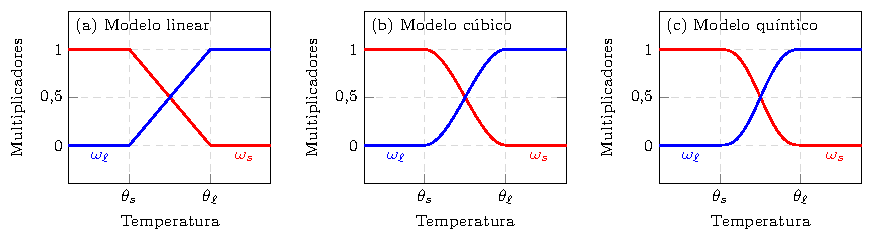
\includegraphics[width=\textwidth]{Figuras/PhaseChangeMultipliers.pdf}
	%\caption*{\textbf{Fonte:} Elaborado pelo autor}
\end{figure}

Neste trabalho, adotamos apenas combinações de multiplicadores que são complementares entre si, ou seja, $\solidMultiplier + \liquidMultiplier = 1$. No entanto, outros tipos de combinações para a fase de transição também podem ser aplicados sem comprometer a consistência do modelo, desde que a continuidade com as fases sólida e líquida seja mantida. As expressões de $\solidMultiplier$ e $\liquidMultiplier$ devem ser avaliadas caso a caso, variando de acordo com o comportamento constitutivo do material analisado na fase de transição.

\vfill

\subsubsection{Implementação numérica}

Na fase de transição, o comportamento constitutivo é análogo ao de um modelo sólido com viscosidade, e a evolução das deformações líquidas é definida puramente pela \cref{eq:evolucao-liquida}. Para a integração temporal dessa lei de evolução, utilizamos o método implícito de Euler, que resulta em
\begin{equation}\label{eq:Rl}
\Rl = \Fl - \Fl\indprev - \Delta t\dfrac{\liquidMultiplier}{2\viscfluid\solidMultiplier\Jl}\Cs\dfrac{\partial\helmholtzs}{\partial\Es}\Fl = \mathbf{0},
\end{equation}
onde $\Fl\indprev$ é o valor de $\Fl$ no passo anterior, e $\Delta t$ é a variação de tempo entre os passos. Nota-se que $\Cs$ e ${\partial\helmholtzs}/{\partial\Es}$ também dependem de $\Fl$. Logo, a \cref{eq:Rl} é um sistema não-linear, sendo resolvido, neste trabalho, pelo método de Newton-Raphson.

As leis de evolução das variáveis internas do sólido também são integradas pela mesma estratégia. Para o modelo viscoelástico-viscoplástico, elas seguem expressões análogas às apresentadas na \cref{sec:solucao-numerica}, adicionando-se apenas o multiplicador sólido. Ou seja:
\begin{align}
& \Rv = \Fv-\Fv\indprev - \dfrac{\Delta t\,\solidMultiplier}{\visc}\mandeleD\Fv = \mathbf{0}, \label{eq:evol-Fv-disc-mushy}\\[0.1cm]
& \Rp = \Fp - \Fp\indprev - \dplastmult\,\solidMultiplier\Np\Fp = \mathbf{0}, \label{eq:evol-Fp-disc-mushy}\\[0.1cm]
& \Rpi = \Fpi - \Fpi\indprev - \dplastmult\,\solidMultiplier\dfrac{\armstrongvisc}{\armstrongstiff}\mandelpeD\Fpi = \mathbf{0}, \label{eq:evol-Fpi-disc-mushy}  \\[0.1cm]
& \Rpvi = \Fpvi - \Fpvi\indprev - \dfrac{\Delta t\,\solidMultiplier}{\visccin}\mandelpveD\Fpvi = \mathbf{0}, \text{\; e}  \label{eq:evol-Fvi-disc-mushy} \\[0.1cm]
& \Renc = \encruamento - \encruamento\indprev - \dplastmult\,\solidMultiplier\sqrt{\dfrac{2}{3}} = 0. \label{eq:evol-encruamento-disc-mushy}
\end{align}
A condição de consistência segue ainda as expressões dadas pelas equações \eqref{eq:comp1} ou \eqref{eq:comp2}, a depender do tipo de plasticidade (independente de taxa ou viscosa).

Uma vez conhecidas as deformações líquidas e sólidas, podemos calcular a tensão pelas equações \eqref{eq:S-mushy} ou \eqref{eq:S-mushy2}. Em teoria, ambas são equivalentes para temperaturas entre $\solidusTemp$ e $\liquidusTemp$, sendo a \cref{eq:S-mushy} indeterminada para $\temp \geq \liquidusTemp$ (pois $\solidMultiplier = 0$), e a \cref{eq:S-mushy2} indeterminada para $\temp \leq \solidusTemp$ (pois $\liquidMultiplier = 0$). No entanto, do ponto de vista computacional, alguns cuidados devem ser tomados também nas proximidades dessas indeterminações. A \cref{eq:S-mushy} tende a causar instabilidades numéricas quando $\solidMultiplier$ é muito pequeno (ou seja, temperaturas muito próximas de $\liquidusTemp$), enquanto a \cref{eq:S-mushy2} tende a causar instabilidades quando $\liquidMultiplier$ é muito pequeno (ou seja, temperaturas muito próximas de $\solidusTemp$). 

Para contornar esse problema, estabelecemos subintervalos específicos de utilização para cada equação. Optamos por dividir o intervalo de temperaturas exatamente na metade, através da seguinte estratégia: para $\liquidFraction \leq 0,5$ (ou $\solidFraction \geq 0,5$), utilizamos a \cref{eq:S-mushy}; para $\liquidFraction > 0,5$ (ou $\solidFraction < 0,5$), utilizamos a \cref{eq:S-mushy2}. Essa estratégia evita divisão por números muito pequenos, minimizando as chances de instabilidades numéricas.

Para o cálculo do operador tangente consistente, devemos adotar uma estratégia que leve em conta a lei de evolução líquida, seguindo procedimentos análogos aos descritos na \cref{sec:operador-vep}. Expressando $\S$ apenas em função de $\E$ e $\Fl$, temos:
\begin{equation}\label{eq:dS-transicao}
\Delta\S \approx \dfrac{\partial\S}{\partial\E}:\Delta\E + \dfrac{\partial\S}{\partial\Fl}:\Delta\Fl.
\end{equation}
Como o resíduo $\Rl$ é nulo para todo passo de tempo, a seguinte aproximação é válida:
\begin{equation}\label{eq:dFl}
\Delta\Rl \approx \dfrac{\partial\Rl}{\partial\E}:\Delta\E + \dfrac{\partial\Rl}{\partial\Fl}:\Delta\Fl \approx \mathbf{0} \quad \Rightarrow\quad \Delta\Fl \approx -\left(\dfrac{\partial\Rl}{\partial\Fl}\right)^{-1}:\dfrac{\partial\Rl}{\partial\E}:\Delta\E.
\end{equation}
Aplicando a \cref{eq:dFl} na \cref{eq:dS-transicao}, temos, enfim
\begin{equation}
\Delta\S \approx \left[\dfrac{\partial\S}{\partial\E} - \dfrac{\partial\S}{\partial\Fl}:\left(\dfrac{\partial\Rl}{\partial\Fl}\right)^{-1}:\dfrac{\partial\Rl}{\partial\E}\right]:\Delta\E.
\end{equation}
Logo, por associação com a \cref{eq:CC-vep-0}, o operador tangente consistente do modelo pode ser definido como
\begin{equation}\label{eq:CC-transicao}
\CC = \dfrac{\partial\S}{\partial\E} - \dfrac{\partial\S}{\partial\Fl}:\left(\dfrac{\partial\Rl}{\partial\Fl}\right)^{-1}:\dfrac{\partial\Rl}{\partial\E},
\end{equation}
onde as derivadas ${\partial\S}/{\partial\E}$ e ${\partial\S}/{\partial\Fl}$ devem ser calculadas a partir da expressão efetivamente utilizada para calcular $\S$. 

Caso $\S$ seja calculado pela \cref{eq:S-mushy}, temos
\begin{align}
&\dfrac{\partial\S}{\partial\E} = \alongTermico^{-1}\CCvol + \alongTermico^{-1}\solidMultiplier^{-1}\Fl^{-1}\left(\CCs:\dfrac{\partial\Es}{\partial\Em}\right)\Fl^{-T}, \text{\quad e} \label{eq:dS_dE1}\\
&\dfrac{\partial\S}{\partial\Fl} = \alongTermico\solidMultiplier^{-1}\left[\Fl^{-1}\left(\CCs:\dfrac{\partial\Es}{\partial\Fl}\right)\Fl^{-T} + \dfrac{\partial\Fl^{-1}}{\partial\Fl}\dfrac{\partial\helmholtzs}{\partial\Es}\Fl^{-T} + \Fl^{-1}\dfrac{\partial\helmholtzs}{\partial\Es}\dfrac{\partial\Fl^{-T}}{\partial\Fl}\right],\label{eq:dS_dFl1}
\end{align}
onde $\CCvol$, $\CCs$ e ${\partial\Es}/{\partial\Em}$ são dados nas \cref{eq:CCaux-solido,eq:dEs_dEm}, e ${\partial\Es}/{\partial\Fl} = \frac{1}{2}{\partial\Cs}/{\partial\Fl}$ pode ser calculado a partir da relação cinemática \eqref{eq:Cs}. 

Caso $\S$ seja calculado pela \cref{eq:S-mushy2}, temos
\begin{align}
&\dfrac{\partial\S}{\partial\E} = \alongTermico^{-1}\CCvol + 4\viscfluid\alongTermico^{-1}\Jl\liquidMultiplier^{-1}\dfrac{\partial\Cm^{-1}}{\partial\Cm}\dotEl\Cl^{-1}, \text{\quad e} \label{eq:dS_dE2}\\
&\dfrac{\partial\S}{\partial\Fl} = 2\viscfluid\alongTermico\Jl\liquidMultiplier^{-1}\left(\Cm^{-1}\dfrac{\partial\dotEl}{\partial\Fl}\Cl^{-1} + \Cm^{-1}\dotEl\dfrac{\partial\Cl^{-1}}{\partial\Cl}:\dfrac{\partial\Cl}{\partial\Fl}\right),\label{eq:dS_dFl2}
\end{align}
onde, para fins de simplificação, desprezamos a derivada de $\Jl$, o que não afeta significativamente o modelo incompressível, uma vez que $\Jl$ tende a ser unitário nesse caso. A derivada ${\partial\dotEl}/{\partial\Fl}$ pode ser aproximada, sem causar perda significativa de convergência, como
\begin{equation}
\dfrac{\partial\dotEl}{\partial\Fl} \approx \dfrac{1}{\Delta t}\dfrac{\partial\El}{\partial\Fl} = \dfrac{1}{2\Delta t}\dfrac{\partial\Cl}{\partial\Fl},
\end{equation}
e, sabendo que $\Cl=\Fl^T\Fl$, podemos calcular ${\partial\Cl}/{\partial\Fl}$ em notação indicial como
\begin{equation}
\dfrac{\partial(\Clind)_{ij}}{\partial(\Flind)_{kl}} = \delta_{il}(\Flind)_{kj} + (\Flind)_{ki}\delta_{jl}.
\end{equation}

No \autoref{quadro:transicao}, apresentamos um resumo esquemático do modelo para a fase de transição, sintetizando os passos discutidos ao longo desta seção.

\begin{quadro}[!htb]
	\centering
	\caption{Resumo esquemático do modelo constitutivo mecânico para a fase de transição ($\solidusTemp < \temp < \liquidusTemp$)}
	\label{quadro:transicao}
	\fbox{%
		\begin{minipage}{\textwidth}
			\vspace{0.4cm}
			
			\begin{enumerate}[label=\arabic*.]
				\item \textbf{Dados:} $\temp$, $\F$, $\Fl\indprev$, $\internalVariables\indprev$
				\item A partir de $\temp$, calcula-se $\alongTermico$ utilizando o modelo de expansão térmica. Disto, temos: 
				
				$\Fm = \alongTermico^{-1}\F \quad\rightarrow\quad \Cm = \Fm^T\Fm \quad\rightarrow\quad \Em = \frac{1}{2}(\Cm-\I)$.
					
				\item Resolve-se a lei de evolução líquida \eqref{eq:Rl} pelo método de Newton-Raphson:
				\begin{enumerate}[label=\alph*)]
					\item Como tentativa inicial, assume-se $\Fl = \Fl\indprev$.
					\item Calcula-se $\Fs = \Fm\Fl^{-1} \quad\rightarrow\quad \Cs = \Fs^T\Fs \quad\rightarrow\quad \Es = \frac{1}{2}(\Cs-\I)$. \label{item:loopRl}
					\item Atualizam-se as variáveis internas do sólido ($\internalVariables$), caso existam, por meio das suas respectivas leis de evolução.
					\item A partir de $\Cs$ e/ou $\Es$, calcula-se ${\partial\helmholtzs}/{\partial\Es}$ utilizando o modelo de sólido.
					\item Calculam-se $\Rl$ e ${\partial\Rl}/{\partial\Fl}$. A correção das deformações líquidas ($\Delta\Fl$) é obtida solucionando-se o sistema linear $\left({\partial\Rl}/{\partial\Fl}\right):\Delta\Fl = -\Rl$.
					\item Se $\|\Delta\Fl\|$ for menor que uma tolerância pré-estabelecida, a solução do sistema é concluída. Caso contrário, $\Delta\Fl$ é adicionada a $\Fl$, e retorna-se ao passo \ref{item:loopRl}.
				\end{enumerate}
				
				
				\item A partir de $\Cm$ e/ou $\Em$, calcula-se ${\partial\helmholtzmvol}/{\partial\Em}$ utilizando o modelo volumétrico. Caso o modelo seja incompressível, deve-se aplicar ainda a condição de incompressibilidade.
				
				\item Se $\liquidFraction \leq 0,5$, utiliza-se a \cref{eq:S-mushy} para o cálculo de $\S$, e as \cref{eq:dS_dE1,eq:dS_dFl1} para o cálculo das derivadas ${\partial\S}/{\partial\E}$ e ${\partial\S}/{\partial\Fl}$.
				
				Se $\liquidFraction > 0,5$, utiliza-se a \cref{eq:S-mushy2} para o cálculo de $\S$, e as \cref{eq:dS_dE2,eq:dS_dFl2} para o cálculo das derivadas ${\partial\S}/{\partial\E}$ e ${\partial\S}/{\partial\Fl}$.
				
				\item Calcula-se $\CC$ pela \cref{eq:CC-transicao}, utilizando as derivadas obtidas no passo anterior.
			\end{enumerate}
			
			\vspace{0.01cm}
		\end{minipage}
	}
\end{quadro}

\subsection{Equação da condução de calor}

Conforme visto nas \cref{sec:solido,sec:liquido,sec:transicao}, podemos expressar a primeira lei da termodinâmica, de forma geral, como
\begin{equation}\label{eq:primeira-lei-mudanca}
\temp \dotentropy + \gradientei\cdot\qi = \dissipationmec + \calorInt,
\end{equation}
ou, utilizando a abordagem baseada em entalpia, discutida na \cref{sec:mudanca-de-fase-termica}:
\begin{equation}
\dotenthalpy + \gradientei\cdot\qi = \dissipationmec + \calorInt,
\end{equation}
onde a taxa de dissipação mecânica é definida como
\begin{equation} \label{eq:dissipation-general}
\dissipationmec = 
\begin{cases}
-\alongTermico^3\left(\dfrac{\partial\helmholtzs}{\partial\internalVariables}:\dotInternalVariables\right) &\text{, para }\temp \leq \solidusTemp, \\
2\viscfluid\alongTermico^3\liquidMultiplier^{-1}\Jl\|\Dl\| - \alongTermico^3\solidMultiplier^{-1}\left(\dfrac{\partial\helmholtzs}{\partial\internalVariables}:\dotInternalVariables\right)&\text{, para }\solidusTemp < \temp < \liquidusTemp, \\
2\viscfluid\alongTermico^3\Jl\|\Dl\|&\text{, para }\temp \geq \liquidusTemp.
\end{cases}
\end{equation}

A taxa de entropia pode ser desenvolvida de forma análoga à apresentada na \cref{sec:conducao-tvep}. Dessa forma, a \cref{eq:primeira-lei-mudanca} resulta novamente na forma da \cref{eq:heat-conduction-final}, diferenciando-se apenas pela adição do calor específico volumétrico latente. Ou seja, a equação da condução de calor é expressa, neste contexto, como
\begin{equation}\label{eq:heat-conduction-final-phasechange}
\left(\volumetricHeatCapacityEff + \volumetricHeatCapacityL\right)\dottemp + \gradientei\cdot\qi = \calorInt + \dissipationMultiplier\dissipationmec - \temp\tmcoupling,
\end{equation}
onde, novamente, o coeficiente $\dissipationMultiplier$ é introduzido para levar em conta o efeito do trabalho frio. O calor específico volumétrico efetivo ($\volumetricHeatCapacityEff$) e o termo de acoplamento termo-mecânico ($\tmcoupling$) são calculados por expressões similares às apresentadas na \cref{sec:conducao-tvep}.

Em geral, fenômenos envolvendo mudança de fase envolvem trocas de calor com grandes variações de temperatura, enquanto os fenômenos mecânicos dissipativos provocam variações de temperatura relativamente pequenas. Dessa forma, nesta seção, optamos por desprezar o efeito da dissipação mecânica e dos termo de acoplamento termo-mecânico na \cref{eq:heat-conduction-final-phasechange}. Além disso, para simplificar os exemplos propostos e dar maior foco ao comportamento constitutivo, desconsideramos a parcela mecânica do calor específico volumétrico, adotando $\volumetricHeatCapacityEff = \volumetricHeatCapacity$, onde $\volumetricHeatCapacity$ é um parâmetro dado do material.

Com essas considerações, a equação da condução de calor resulta na forma puramente térmica apresentada na \cref{eq:cond-enthalpy}, devendo ser utilizadas as mesmas estratégias de implementação numérica discutidas na \cref{sec:implementacao-mudanca-fase}. Vale ressaltar que isso não elimina a influência do problema mecânico sobre o térmico, especialmente em casos com grandes deformações, uma vez que alterações significativas na configuração do domínio impactam a distribuição de temperatura. Para o acoplamento termo-mecânico, seguimos utilizando o método bloco-iterativo descrito na \cref{subsec:acoplamento}.


\subsection{Exemplos numéricos}

Nesta seção, são propostos exemplos numéricos representativos para caracterizar o comportamento constitutivo do modelo proposto, bem como verificar a sua consistência. Os exemplos iniciais (subseções \ref{subsec:local1} e \ref{subsec:local2}) abordam problemas locais, ou pontuais, onde estamos interessados apenas em calcular a tensão a partir da deformação, da temperatura e de suas respectivas taxas, sem considerar o domínio ao redor. Já nos demais exemplos, o modelo constitutivo é incorporado ao Método dos Elementos Finitos, permitindo a análise de problemas mais complexos com domínios bidimensionais ou tridimensionais.

\subsubsection{Problema local de deformação monotônica com solidificação}\label{subsec:local1}

Neste exemplo, estamos interessados em analisar o comportamento constitutivo de um ponto comprimido uniaxialmente ao mesmo tempo que sofre mudança da fase líquida para a sólida. Consideramos que a componente uniaxial da deformação linear de engenharia ($\defLinearind_{11} = \Find_{11}-1$) varia linearmente entre $0$ e $-0,4$ com uma taxa constante de $\dotDefLinearind_{11} = -0,4/t_\text{max}$, onde $t_\text{max}$ é o tempo máximo da análise. Simultaneamente, aplicamos uma temperatura prescrita variando linearmente entre $50\,^{\circ}$C e $0\,^{\circ}$C. Consideramos três diferentes valores de $t_\text{max}$: $25$, $5$ e $1$ s, resultando em taxas distintas de deformação e temperatura. Em todos os casos, aplica-se uma discretização temporal com $400$ passos de tempo.

Para a fase líquida, adotamos o modelo de fluido Newtoniano incompressível, e para a fase sólida, um material hiperelástico neo-Hookeano, também incompressível. Os parâmetros relevantes para esse problema são dispostos na \cref{tab:parametros-phasechangemonotonic}. Observa-se que, por ser um material incompressível, o parâmetro $\lame$ do modelo neo-Hookeano não se aplica. Além disso, não consideramos expansão/contração térmica neste caso.

\begin{table}[!htb]
	\centering
	\caption{Parâmetros do material utilizado nas análises de problemas locais com mudança de fase}
	\footnotesize
	\label{tab:parametros-phasechangemonotonic}
	{\renewcommand{\arraystretch}{1.1}
		\begin{tabular}{cccc}
			\hline
			\rowcolor{LightGray}
			$\viscfluid$ (MPa$\cdot$s) & $\G$ (MPa) & $\solidusTemp$ ($^{\circ}$C) & $\liquidusTemp$ ($^{\circ}$C)  \\  
			$0,1$ & $1$ & $15$ & $30$  \\ \hline
		\end{tabular}
	}
	%\caption*{\textbf{Fonte:} Elaborado pelo autor}
\end{table}

Os resultados para os três casos de $t_\text{max}$ são apresentados nas  \cref{fig:PhaseChangeMonotonicStrainLiquidToSolid-t25,fig:PhaseChangeMonotonicStrainLiquidToSolid-t5,fig:PhaseChangeMonotonicStrainLiquidToSolid-t1}. Em cada caso, são mostrados os gráficos de tensão de Cauchy uniaxial ($\cauchyind_{11}$), e os componentes sólido e líquido de $\Find_{11}$, com as fases do material indicadas nos seus respectivos intervalos de tempo.

O principal ponto a ser analisado neste problema é a continuidade da resposta obtida. Uma vez que cada fase é governada por um modelo constitutivo diferente, cabe verificar se a transição entre as fases ocorre de forma suave. Para isso, são testados os três modelos de multiplicadores dispostos na \cref{tab:modelos} para a fase de transição.

No caso com $t_\text{max}=25$ s (\cref{fig:PhaseChangeMonotonicStrainLiquidToSolid-t25}), a taxa de deformação é muito pequena, resultando em tensões significativamente menores na fase líquida em comparação com a fase sólida. Nesse caso, não há descontinuidades perceptíveis nos gráficos, e a transição ocorre de forma suave para todos os modelos de multiplicadores, embora as respostas variem entre esses modelos a partir da fase de transição, como esperado.

\begin{figure}[htb]
	\centering
	\caption{Gráficos de (a) tensão de Cauchy uniaxial e (b) componentes sólida e líquida de $\Find_{11}$, para os casos com $\dotDefLinearind_{11} = -0,016$ s$^{-1}$ e $\dottemp = -2\, ^{\circ}$C/s}
	\label{fig:PhaseChangeMonotonicStrainLiquidToSolid-t25}
	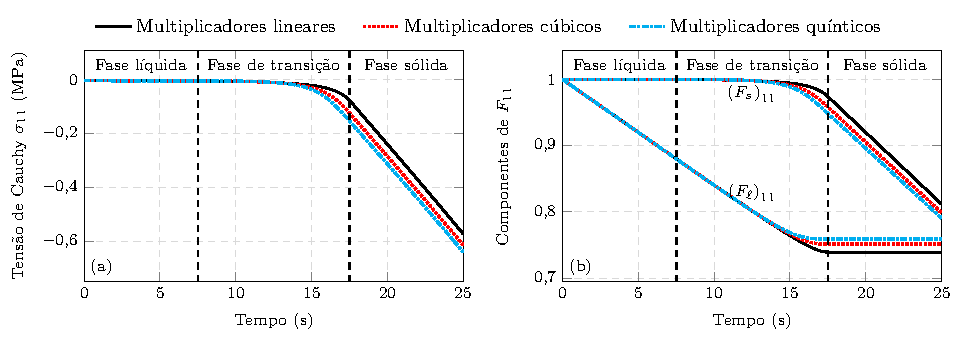
\includegraphics[scale=1.0]{Figuras/PhaseChangeMonotonic/PhaseChangeMonotonicStrainLiquidToSolid-t25.pdf}
	%\caption*{\textbf{Fonte:} Elaborado pelo autor}
\end{figure}

No caso com $t_\text{max}=5$ s (\cref{fig:PhaseChangeMonotonicStrainLiquidToSolid-t5}), surge uma pequena descontinuidade nas tensões entre a fase líquida e a de transição para o modelo com multiplicadores lineares, apesar de essa descontinuidade apenas ser perceptível no gráfico ampliado. Já nos casos com multiplicadores cúbicos e quínticos, a transição das tensões se mostra suave mesmo no gráfico ampliado.

\begin{figure}[htb]
	\centering
	\caption{Gráficos de (a) tensão de Cauchy uniaxial e (b) componentes sólida e líquida de $\Find_{11}$, para os casos com $\dotDefLinearind_{11} = -0,08$ s$^{-1}$ e $\dottemp = -10\, ^{\circ}$C/s}
	\label{fig:PhaseChangeMonotonicStrainLiquidToSolid-t5}
	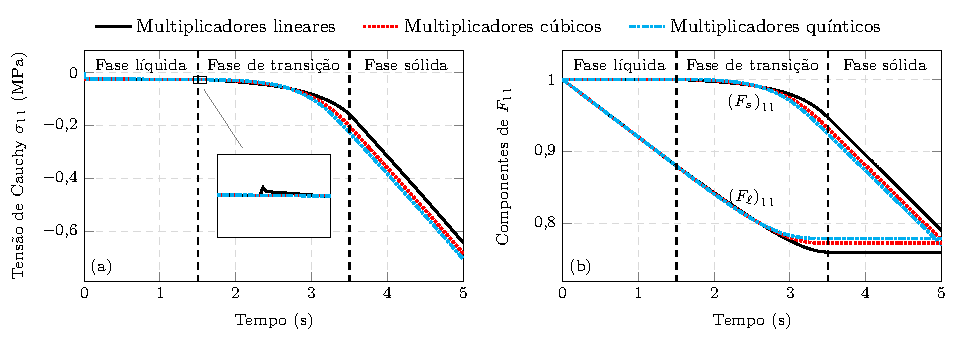
\includegraphics[scale=1.0]{Figuras/PhaseChangeMonotonic/PhaseChangeMonotonicStrainLiquidToSolid-t5.pdf}
	%\caption*{\textbf{Fonte:} Elaborado pelo autor}
\end{figure}

Por fim, no caso com $t_\text{max}=1$ s (\cref{fig:PhaseChangeMonotonicStrainLiquidToSolid-t1}), a descontinuidade das tensões para o modelo com multiplicadores lineares se torna mais expressiva, mostrando irregularidades no início da fase de transição. Além disso, podemos observar uma quebra de suavidade das tensões, ou seja, uma mudança abrupta na inclinação da curva, entre as fases de transição e sólida. Para o modelo com multiplicadores cúbicos, a resposta é contínua, mas também é possível perceber uma quebra de suavidade entre as fases líquida e de transição. Já o modelo quíntico permanece contínuo e suave ao longo de todas as transições.

\begin{figure}[htb]
	\centering
	\caption{Gráficos de (a) tensão de Cauchy uniaxial e (b) componentes sólida e líquida de $\Find_{11}$, para os casos com $\dotDefLinearind_{11} = -0,4$ s$^{-1}$ e $\dottemp = -50\, ^{\circ}$C/s}
	\label{fig:PhaseChangeMonotonicStrainLiquidToSolid-t1}
	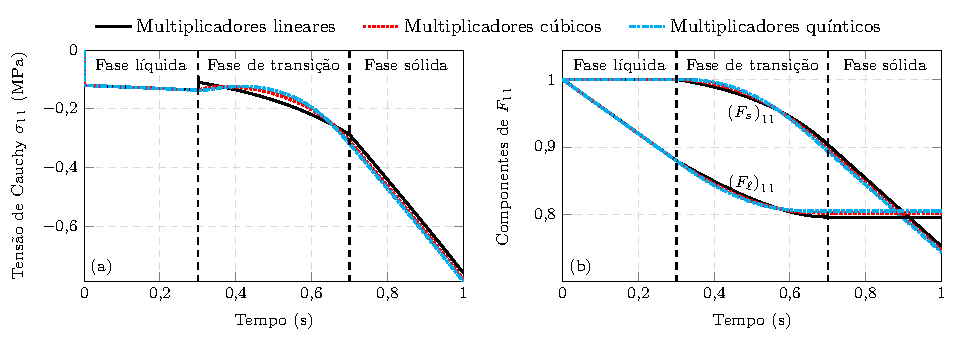
\includegraphics[scale=1.0]{Figuras/PhaseChangeMonotonic/PhaseChangeMonotonicStrainLiquidToSolid-t1.pdf}
	%\caption*{\textbf{Fonte:} Elaborado pelo autor}
\end{figure}

Os gráficos das componentes sólida e líquida de $\Find_{11}$ mostram evoluções consistentes com suas respectivas fases, e mantêm-se contínuos em todos os casos, independentemente do modelo adotado para os multiplicadores. A única quebra de suavidade perceptível ocorre no gráfico de $(\Fsind)_{11}$ para $t_\text{max}=1$, entre as fases líquida e de transição, coincidindo com o ponto de descontinuidade no gráfico de tensão.

Vale observar que quebras de continuidade ou de suavidade não necessariamente indicam uma falha no modelo, mas sim uma característica intrínseca do mesmo. Ao aplica-lo em um contexto prático, é importante verificar o comportamento do material analisado, e utilizar o modelo que melhor se adeque a esse comportamento, seja ele contínuo ou não. Neste trabalho, caracterizamos apenas algumas opções de multiplicadores, mas as possibilidades de ajustes são infinitas.



\subsubsection{Problema local de deformação monotônica com fusão}\label{subsec:local2}

Nesta subseção, apresentamos um exemplo similar ao anterior, porém, com mudança da fase sólida para a líquida. Mantemos as deformações prescritas, os parâmetros do material (\cref{tab:parametros-phasechangemonotonic}), os tempos máximos de análise, e a discretização temporal, mas neste caso variamos as temperaturas linearmente de $0\,^{\circ}$C para $50\,^{\circ}$C ao longo do tempo.

Os resultados para os três casos de $t_\text{max}$ são apresentados nas  \cref{fig:PhaseChangeMonotonicStrainSolidToLiquid-t25,fig:PhaseChangeMonotonicStrainSolidToLiquid-t5,fig:PhaseChangeMonotonicStrainSolidToLiquid-t1}. Dado que as tensões na fase sólida são maiores em comparação com a fase líquida, e aumentam progressivamente com as deformações, é natural observar uma alteração no perfil de transição em relação ao exemplo anterior. Embora a tendência seja a diminuição da tensão ao longo da fase de transição, ela atinge o seu valor de pico nessa fase. Esses picos se mostram mais acentuados nos modelos cúbicos e quínticos.

\begin{figure}[!htb]
	\centering
	\caption{Gráficos de (a) tensão de Cauchy uniaxial e (b) componentes sólida e líquida de $\Find_{11}$, para os casos com $\dotDefLinearind_{11} = -0,016$ s$^{-1}$ e $\dottemp = 2\, ^{\circ}$C/s}
	\label{fig:PhaseChangeMonotonicStrainSolidToLiquid-t25}
	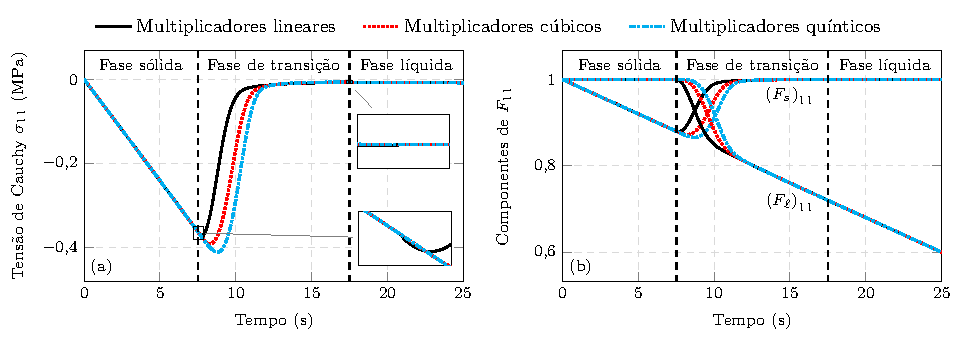
\includegraphics[scale=1.0]{Figuras/PhaseChangeMonotonic/PhaseChangeMonotonicStrainSolidToLiquid-t25.pdf}
	%\caption*{\textbf{Fonte:} Elaborado pelo autor}
\end{figure}

\begin{figure}[!htb]
	\centering
	\caption{Gráficos de (a) tensão de Cauchy uniaxial e (b) componentes sólida e líquida de $\Find_{11}$, para os casos com $\dotDefLinearind_{11} = -0,08$ s$^{-1}$ e $\dottemp = 10\, ^{\circ}$C/s}
	\label{fig:PhaseChangeMonotonicStrainSolidToLiquid-t5}
	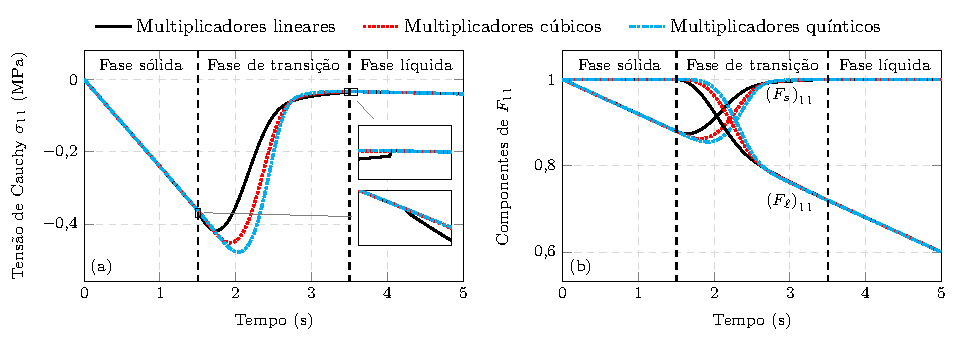
\includegraphics[scale=1.0]{Figuras/PhaseChangeMonotonic/PhaseChangeMonotonicStrainSolidToLiquid-t5.pdf}
	%\caption*{\textbf{Fonte:} Elaborado pelo autor}
\end{figure}

\begin{figure}[!htb]
	\centering
	\caption{Gráficos de (a) tensão de Cauchy uniaxial e (b) componentes sólida e líquida de $\Find_{11}$, para os casos com $\dotDefLinearind_{11} = -0,4$ s$^{-1}$ e $\dottemp = 50\, ^{\circ}$C/s}
	\label{fig:PhaseChangeMonotonicStrainSolidToLiquid-t1}
	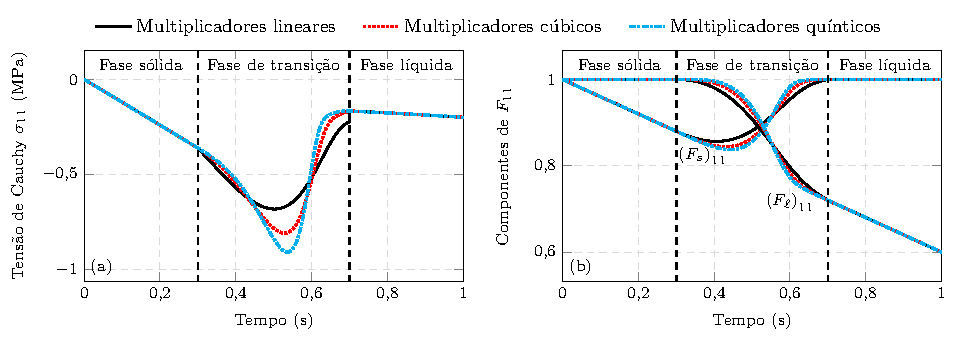
\includegraphics[scale=1.0]{Figuras/PhaseChangeMonotonic/PhaseChangeMonotonicStrainSolidToLiquid-t1.pdf}
	%\caption*{\textbf{Fonte:} Elaborado pelo autor}
\end{figure}

Nos gráficos de $(\Fsind)_{11}$ e $(\Flind)_{11}$, observamos novamente um comportamento consistente, com a componente sólida diminuindo gradativamente até zero à medida que a mudança de fase avança, enquanto a componente líquida tende à deformação total.

As descontinuidades e quebras de suavidade são análogas às observadas no exemplo anterior, ocorrendo nas mesmas transições de fases para os mesmos casos. A única diferença é o caso com $t_\text{max} = 25$ s (\cref{fig:PhaseChangeMonotonicStrainSolidToLiquid-t25}), onde a mudança de inclinação da curva de tensão entre as fases sólida e de transição é evidente no gráfico ampliado do modelo com multiplicadores lineares. Por outro lado, a descontinuidade entre as fases de transição e líquida nesse mesmo gráfico permanece praticamente imperceptível, mesmo na versão ampliada, ao contrário dos casos com $t_\text{max} = 5$ s e $t_\text{max} = 1$ s.


%\subsubsection{Problema local de relaxação com solidificação}\label{subsec:local3}
%
%\begin{figure}[!htb]
%	\centering
%	\caption{Gráficos de (a) tensão de Cauchy uniaxial e (b) componentes sólida e líquida de $\Find_{11}$, para relaxação com $\dottemp = -10\, ^{\circ}$C/s}
%	\label{fig:PhaseChangeRelaxationLiquidToSolid-t5}
%	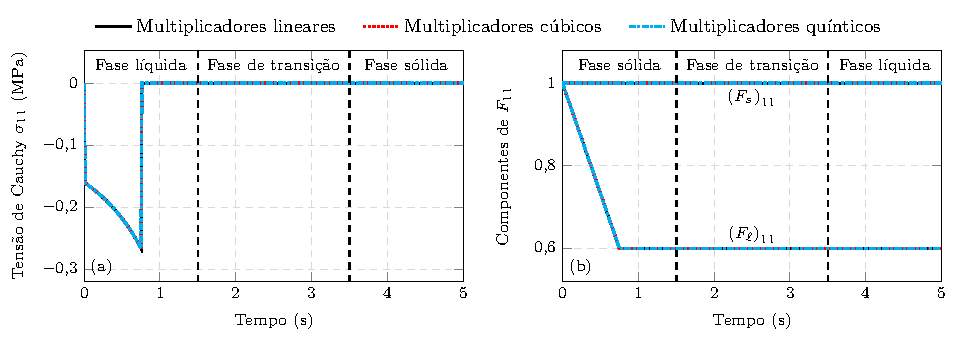
\includegraphics[scale=1.0]{Figuras/PhaseChangeMonotonic/PhaseChangeRelaxationLiquidToSolid-t5.pdf}
%	%\caption*{\textbf{Fonte:} Elaborado pelo autor}
%\end{figure}
%
%\subsubsection{Problema local de relaxação com fusão}\label{subsec:local4}
%
%\begin{figure}[!htb]
%	\centering
%	\caption{Gráficos de (a) tensão de Cauchy uniaxial e (b) componentes sólida e líquida de $\Find_{11}$, para relaxação com $\dottemp = 2\, ^{\circ}$C/s}
%	\label{fig:PhaseChangeRelaxationSolidToLiquid-t25}
%	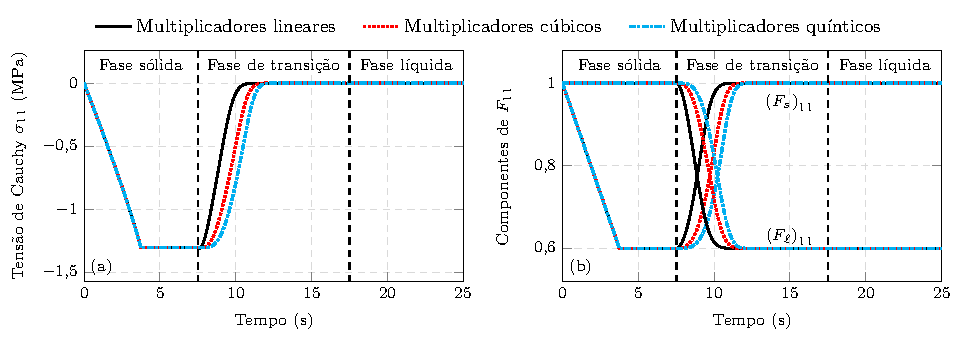
\includegraphics[scale=1.0]{Figuras/PhaseChangeMonotonic/PhaseChangeRelaxationSolidToLiquid-t25.pdf}
%	%\caption*{\textbf{Fonte:} Elaborado pelo autor}
%\end{figure}
%
%\begin{figure}[!htb]
%	\centering
%	\caption{Gráficos de (a) tensão de Cauchy uniaxial e (b) componentes sólida e líquida de $\Find_{11}$, para relaxação com $\dottemp = 10\, ^{\circ}$C/s}
%	\label{fig:PhaseChangeRelaxationSolidToLiquid-t5}
%	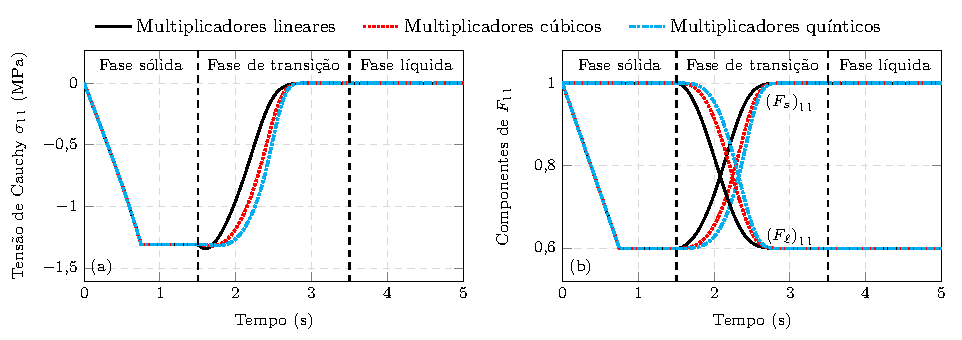
\includegraphics[scale=1.0]{Figuras/PhaseChangeMonotonic/PhaseChangeRelaxationSolidToLiquid-t5.pdf}
%	%\caption*{\textbf{Fonte:} Elaborado pelo autor}
%\end{figure}
%
%\begin{figure}[!htb]
%	\centering
%	\caption{Gráficos de (a) tensão de Cauchy uniaxial e (b) componentes sólida e líquida de $\Find_{11}$, para relaxação com $\dottemp = 50\, ^{\circ}$C/s}
%	\label{fig:PhaseChangeRelaxationSolidToLiquid-t1}
%	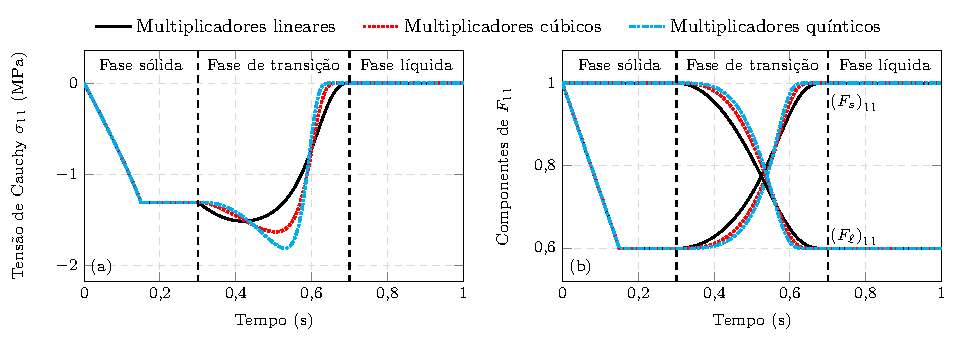
\includegraphics[scale=1.0]{Figuras/PhaseChangeMonotonic/PhaseChangeRelaxationSolidToLiquid-t1.pdf}
%	%\caption*{\textbf{Fonte:} Elaborado pelo autor}
%\end{figure}

\subsubsection{Prensagem de cilindro solidificado}

Este exemplo possui como principal objetivo verificar a consistência cinemática do modelo em uma análise bidimensional. Inicialmente, simulamos um líquido com formato retangular que, sob a ação de uma tensão superficial, torna-se eventualmente um círculo/cilindro. Após assumir esse formato, o material é solidificado e submetido à prensagem por uma parede rígida móvel. Em uma outra análise, simulamos um sólido já no formato cilíndrico com raio equivalente, submetido à mesma prensagem. Durante a fase sólida, os dois casos tratam-se essencialmente do mesmo problema, mas utilizam configurações iniciais diferentes -- retangular líquida no primeiro, e circular sólida no segundo. Para que o modelo de mudança de fase seja consistente, é necessário que as duas respostas coincidam apesar das diferentes referências Lagrangianas.

Os dados do exemplo para as duas análises são dispostos na \cref{fig:PhaseChangeConsistencyTest2D}, incluindo as malhas utilizadas. Aproveitando a simetria dos problemas, apenas um quadrante das geometrias são discretizadas, com as devidas condições de contorno aplicadas nas interfaces dos eixos de simetria. De forma a simplificar o exemplo e mantê-lo direcionado aos objetivos propostos, desconsideramos o peso próprio e demais forças externas além da tensão superficial, bem como o efeito da contração térmica. Aplica-se a estabilização PSPG com $\multiplierpspg = 1$, e utiliza-se o integrador de Newmark-$\beta$ com parâmetros $\betanewmark = 1$ e $\gammanewmark = 1,5$.

Para o caso com solidificação, aplica-se uma temperatura prescrita constante ao longo do domínio, dispensando a necessidade de resolver a equação da condução de calor. Essa temperatura é reduzida de $650\,^{\circ}$C para $325\,^{\circ}$C ao longo de $2$ segundos, o que corresponde aproximadamente ao instante da mudança de fase, já que a temperatura de solidificação é cerca de $327\,^{\circ}$C. Esse intervalo de tempo é suficiente para que o líquido se estabilize na configuração cilíndrica. Como o intervalo entre $\solidusTemp$ e $\liquidusTemp$ é muito pequeno, o modelo constitutivo da fase de transição é irrelevante para esse problema. Após os $2$ segundos iniciais, é aplicado um deslocamento prescrito progressivo na parede rígida, que entra em contato com o sólido, provocando a prensagem. 

No caso puramente sólido, desconsidera-se a variação térmica, e mantem-se uma configuração praticamente estática nos $2$ segundos iniciais antes do início da prensagem. Para garantir a objetividade da comparação, a tensão superficial permanece sendo aplicada neste caso, apesar de seu efeito ser desprezível no sólido.


\begin{figure}[!htb]
	\centering
	\caption{Dados para o exemplo de prensagem de cilindro solidificado}
	\label{fig:PhaseChangeConsistencyTest2D}
	{\small
		\noindent\shadowbox{
			\parbox{15.3cm}{
				\setlength{\columnseprule}{1pt}
				\vspace{-0.2cm}
				{\centering\begin{center}
						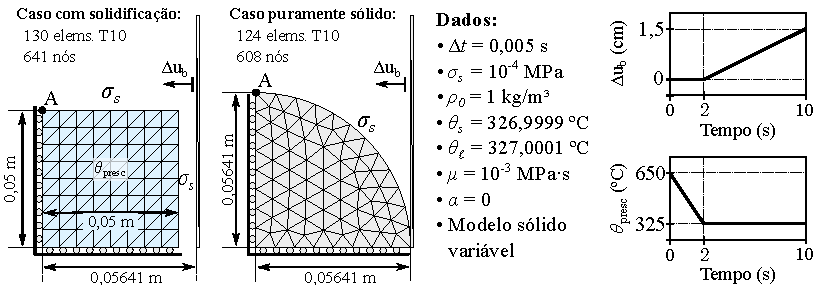
\includegraphics[scale=1.1]{Figuras/PhaseChangeConsistencyTest2D/PhaseChangeConsistencyTest2D.pdf}
					\end{center}\par}
				\vspace{-0.2cm}
			}
		}
	}	
	%\caption*{\textbf{Fonte:} Elaborado pelo autor}
\end{figure}
\vspace{-0.2cm}
Para demonstrar a consistência da formulação em diferentes cenários, consideramos dois materiais para a fase sólida. No primeiro, utilizamos um modelo hiperelástico incompressível com $\G = 160$ MPa. No segundo cenário, aplicamos o material PTFE, utilizando o modelo viscoelástico-viscoplástico com parâmetros calibrados na \cref{tab:parametros-PTFE}. O modelo do PTFE neste caso é adaptado para o caso incompressível, o que significa que a contribuição volumétrica associada ao parâmetro 
$\lame$ é ignorada e substituída pela condição de incompressibilidade.

Na \cref{fig:PhaseChangeConsistencyTest2D-DisplacementAndPressure}(a), os gráficos mostram a evolução da coordenada $x_2$ (eixo vertical) no ponto A, situado na extremidade superior da configuração circular. A origem do eixo $x_2$ é tomada no centro do círculo. Na \cref{fig:PhaseChangeConsistencyTest2D-DisplacementAndPressure}(b), os gráficos mostram a evolução da força de reação horizontal, calculada como a resultante das forças de reação em todos os nós restritos horizontalmente. A comparação das curvas nesses gráficos revela uma ótima correspondência entre os casos com solidificação e o puramente sólido, para ambos os materiais considerados. Naturalmente, essa correspondência é avaliada apenas após os $2$ segundos iniciais da análise, onde os problemas analisados passam a coincidir.

\begin{figure}[!htb]
	\centering
	\caption{Gráficos de (a) coordenada $\xind_2$ no ponto A e (b) força de reação horizontal para o problema de prensagem de cilindro solidificado}
	\label{fig:PhaseChangeConsistencyTest2D-DisplacementAndPressure}
	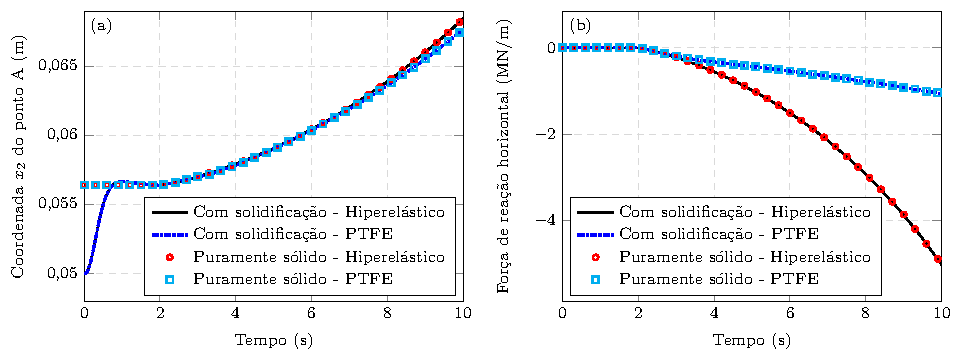
\includegraphics[scale=1.0]{Figuras/PhaseChangeConsistencyTest2D/DisplacementAndPressure.pdf}
	%\caption*{\textbf{Fonte:} Elaborado pelo autor}
\end{figure}

As configurações deformadas dos problemas, com componente $\cauchyind_{11}$ da tensão de Cauchy em mapa de cores, estão apresentadas nas \cref{fig:PhaseChangeConsistencyTest2D-Elastic,fig:PhaseChangeConsistencyTest2D-PTFE} para o material hiperelástico e o PTFE, respectivamente. Em ambas as figuras, são mostradas lado a lado as configurações do caso puramente sólido (à esquerda, espelhado) e do caso com solidificação (à direita), permitindo uma comparação visual dos resultados nos instantes selecionados. Mesmo com as malhas distintas, é possível observar uma excelente concordância em todos os casos a partir de $2$ segundos.

\begin{figure}[!htb]
	\centering
	\caption{Configurações deformadas para o material hiperelástico, com $\cauchyind_{11}$ em mapa de cores}
	\label{fig:PhaseChangeConsistencyTest2D-Elastic}
	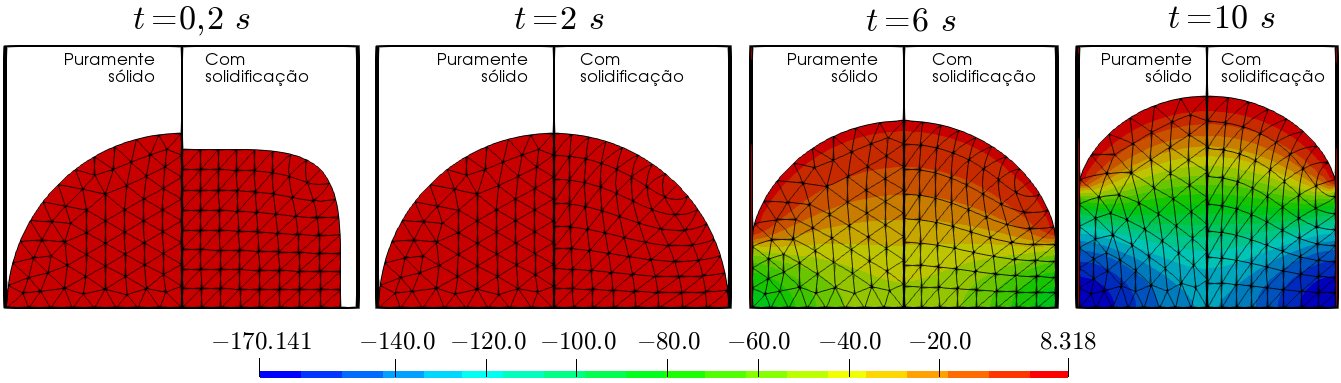
\includegraphics[width=\textwidth]{Figuras/PhaseChangeConsistencyTest2D/Elastic.png}
	%\caption*{\textbf{Fonte:} Elaborado pelo autor}
\end{figure}

\begin{figure}[!htb]
	\centering
	\caption{Configurações deformadas para o PTFE, com $\cauchyind_{11}$ em mapa de cores}
	\label{fig:PhaseChangeConsistencyTest2D-PTFE}
	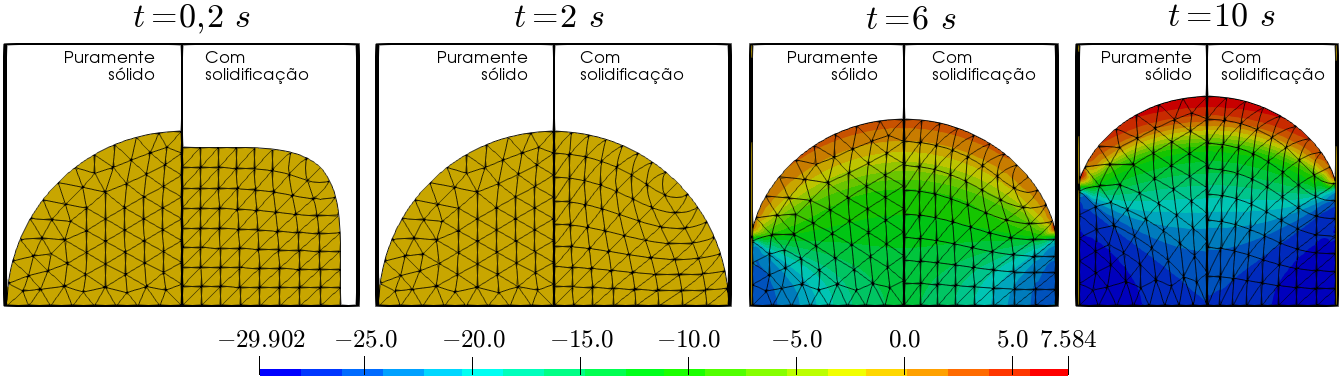
\includegraphics[width=\textwidth]{Figuras/PhaseChangeConsistencyTest2D/PTFE.png}
	%\caption*{\textbf{Fonte:} Elaborado pelo autor}
\end{figure}



\subsubsection{Prensagem de esfera solidificada}

Similarmente ao exemplo anterior, este caso busca verificar a consistência cinemática do modelo, mas desta vez em uma análise tridimensional. Simulamos um líquido em formato cúbico que, sob a ação de uma tensão superficial, eventualmente se transforma em uma esfera. Após assumir essa forma, o material é solidificado e submetido à prensagem por uma parede rígida móvel. Novamente, comparamos a resposta com um caso puramente sólido, onde, desde o início da análise, o material já possui formato esférico de raio equivalente e encontra-se na fase sólida.

Na \cref{fig:PhaseChangeConsistencyTest3D}, são apresentadas as geometrias, malhas, e condições de contorno para cada caso. Devido à simetria do problema, apenas um octante é discretizado, sendo aplicadas as devidas condições de contorno nos eixos de simetria. Os demais dados da análise, incluindo os materiais utilizados e temperaturas prescritas, são exatamente iguais aos do exemplo anterior. Porém, neste caso, analisamos também um cenário com contração térmica, aplicando o modelo exponencial com $\coefExp = 1,25\cdot 10^{-4}\,^{\circ}$C$^{-1}$. Para permitir a comparação entre os casos com solidificação e o puramente sólido no cenário com contração térmica, a mesma variação de temperatura é aplicada em ambos durante os $2$ segundos iniciais da análise.

\begin{figure}[!htb]
	\centering
	\caption{Geometrias para o exemplo de prensagem de esfera solidificada}
	\label{fig:PhaseChangeConsistencyTest3D}
	{\small
		\noindent\shadowbox{
			\parbox{15.3cm}{
				\setlength{\columnseprule}{1pt}
				\vspace{-0.3cm}
				{\centering\begin{center}
						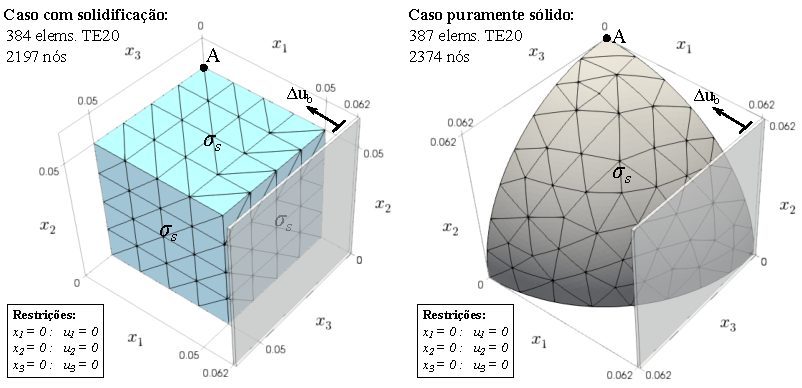
\includegraphics[scale=1.1]{Figuras/PhaseChangeConsistencyTest3D/PhaseChangeConsistencyTest3D.pdf}
					\end{center}\par}
				\vspace{-0.2cm}
			}
		}
	}	
	%\caption*{\textbf{Fonte:} Elaborado pelo autor}
\end{figure}

Assim como no exemplo anterior, utilizamos como base de comparação os gráficos da coordenada $x_2$ no ponto A e força de reação horizontal (eixo $x_1$) ao longo do tempo. Esses gráficos são mostrados nas \cref{fig:PhaseChangeConsistencyTest3D-DisplacementAndReaction-a0,fig:PhaseChangeConsistencyTest3D-DisplacementAndReaction-a125e-4} para os casos com $\coefExp = 0$ e $\coefExp = 1,25\cdot 10^{-4}\,^{\circ}$C$^{-1}$, respectivamente. O primeiro caso apresenta perfis similares aos do exemplo anterior. Já no segundo caso, podemos perceber uma redução da coordenada $x_2$, devido ao efeito da contração térmica. Naturalmente, a contração também ocorre no eixo $x_1$, o que retarda o instante no qual a parede entra em contato com o sólido, consequentemente alterando a evolução das forças de reação.

Novamente, os gráficos demonstram uma excelente correspondência entre os casos com solidificação e puramente sólido, a partir dos $2$ segundos iniciais, independentemente do material e do coeficiente $\coefExp$ adotados. Isso sugere a consistência do modelo proposto de mudança de fase, mesmo em problemas tridimensionais sob diferentes condições.

\begin{figure}[!htb]
	\centering
	\caption{Gráficos de (a) coordenada $\xind_2$ no ponto A e (b) força de reação horizontal para o problema de prensagem de esfera solidificada com $\coefExp = 0$}
	\label{fig:PhaseChangeConsistencyTest3D-DisplacementAndReaction-a0}
	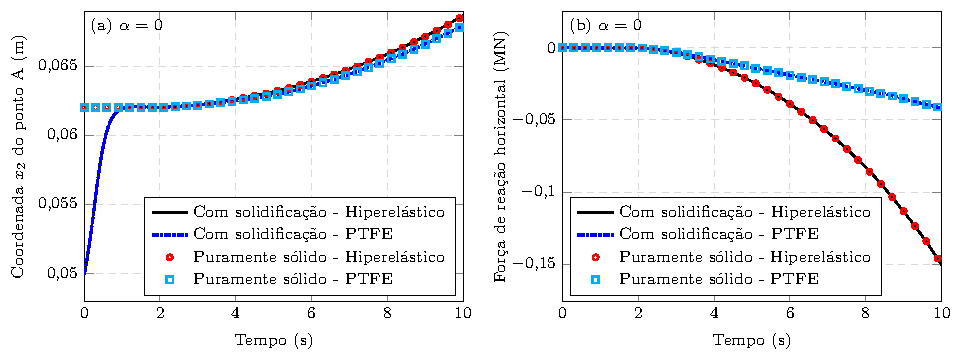
\includegraphics[scale=1.0]{Figuras/PhaseChangeConsistencyTest3D/DisplacementAndReaction-a0.pdf}
	%\caption*{\textbf{Fonte:} Elaborado pelo autor}
\end{figure}

\begin{figure}[!htb]
	\centering
	\caption{Gráficos de (a) coordenada $\xind_2$ no ponto A e (b) força de reação horizontal para o problema de prensagem de esfera solidificada com $\coefExp = 1,25\cdot 10^{-4}\,^{\circ}$C$^{-1}$}
	\label{fig:PhaseChangeConsistencyTest3D-DisplacementAndReaction-a125e-4}
	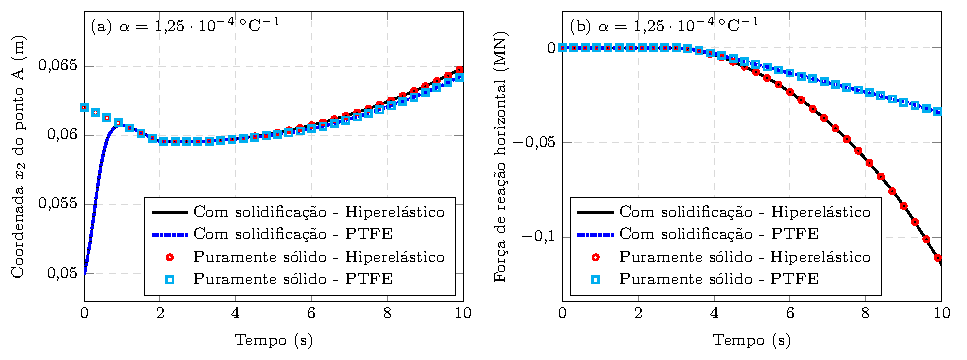
\includegraphics[scale=1.0]{Figuras/PhaseChangeConsistencyTest3D/DisplacementAndReaction-a1e-4.pdf}
	%\caption*{\textbf{Fonte:} Elaborado pelo autor}
\end{figure}

Nas \cref{fig:PhaseChangeConsistencyTest3D-Elastic,fig:PhaseChangeConsistencyTest3D-Elastic-a125e-4,fig:PhaseChangeConsistencyTest3D-PTFE,fig:PhaseChangeConsistencyTest3D-PTFE-a125e-4}, apresentamos as configurações deformadas para todas as variações consideradas de materiais e dos coeficientes $\coefExp$. Em cada instante de tempo selecionado, mostramos o caso puramente sólido à esquerda, e o caso com solidificação à direita (espelhado), permitindo uma comparação visual direta. Nos mapas de cores, são exibidos os valores da pressão, em MPa. Novamente, para instantes a partir de $2$ segundos, as figuras mostram excelente concordância entre os dois casos, apesar das diferentes malhas adotadas.

A parede rígida foi omitida das figuras para não obstruir a visualização dos resultados, mas o efeito da prensagem é evidente nos instantes de $6$ e $10$ segundos. O impacto da contração térmica nas configurações deformadas é sutil, mas a variação no volume pode ser percebida ao comparar as configurações do caso puramente sólido nos instantes de $0,2$ e $2$ segundos das \cref{fig:PhaseChangeConsistencyTest3D-Elastic-a125e-4,fig:PhaseChangeConsistencyTest3D-PTFE-a125e-4}.

\begin{figure}[!htb]
	\centering
	\caption{Configurações deformadas para material hiperelástico e $\coefExp = 0$, com caso puramente sólido à esquerda e com solidificação à direita, e pressão (MPa) em mapa de cores}
	\label{fig:PhaseChangeConsistencyTest3D-Elastic}
	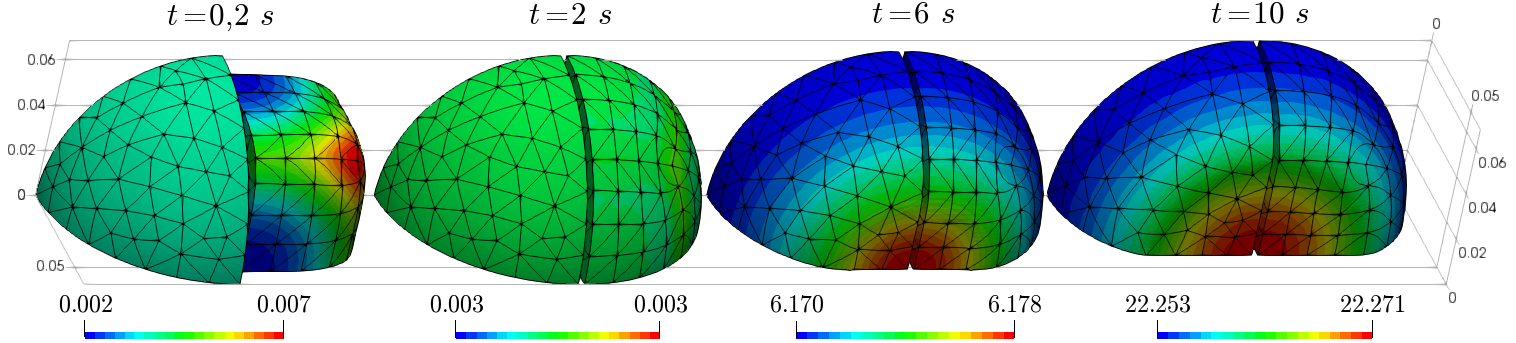
\includegraphics[width=\textwidth]{Figuras/PhaseChangeConsistencyTest3D/Elastic-a0.png}
	%\caption*{\textbf{Fonte:} Elaborado pelo autor}
\end{figure}

\begin{figure}[!htb]
	\centering
	\caption{Configurações deformadas para material hiperelástico e $\coefExp = 1,25\cdot 10^{-4}\,^{\circ}$C$^{-1}$, com caso puramente sólido à esquerda e com solidificação à direita, e pressão (MPa) em mapa de cores}
	\label{fig:PhaseChangeConsistencyTest3D-Elastic-a125e-4}
	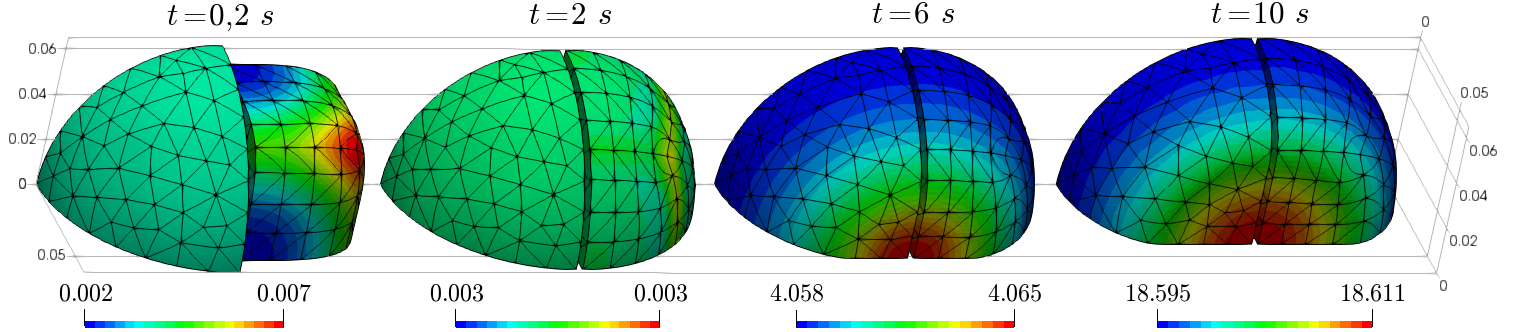
\includegraphics[width=\textwidth]{Figuras/PhaseChangeConsistencyTest3D/Elastic-a125e-4.png}
	%\caption*{\textbf{Fonte:} Elaborado pelo autor}
\end{figure}

\begin{figure}[!htb]
	\centering
	\caption{Configurações deformadas para PTFE e $\coefExp = 0$, com caso puramente sólido à esquerda e com solidificação à direita, e pressão (MPa) em mapa de cores}
	\label{fig:PhaseChangeConsistencyTest3D-PTFE}
	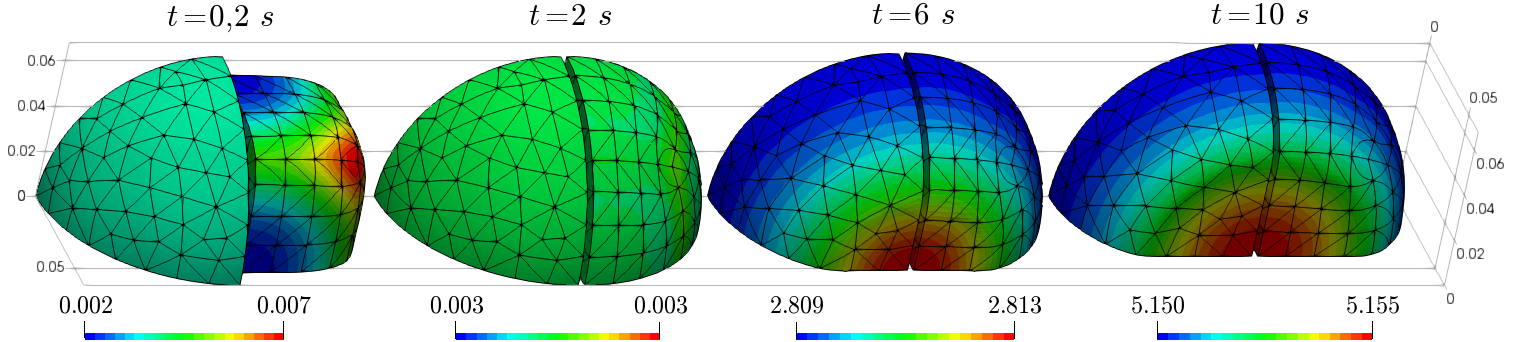
\includegraphics[width=\textwidth]{Figuras/PhaseChangeConsistencyTest3D/PTFE-a0.png}
	%\caption*{\textbf{Fonte:} Elaborado pelo autor}
\end{figure}

\begin{figure}[!htb]
	\centering
	\caption{Configurações deformadas para PTFE e $\coefExp = 1,25\cdot 10^{-4}\,^{\circ}$C$^{-1}$, com caso puramente sólido à esquerda e com solidificação à direita, e pressão (MPa) em mapa de cores}
	\label{fig:PhaseChangeConsistencyTest3D-PTFE-a125e-4}
	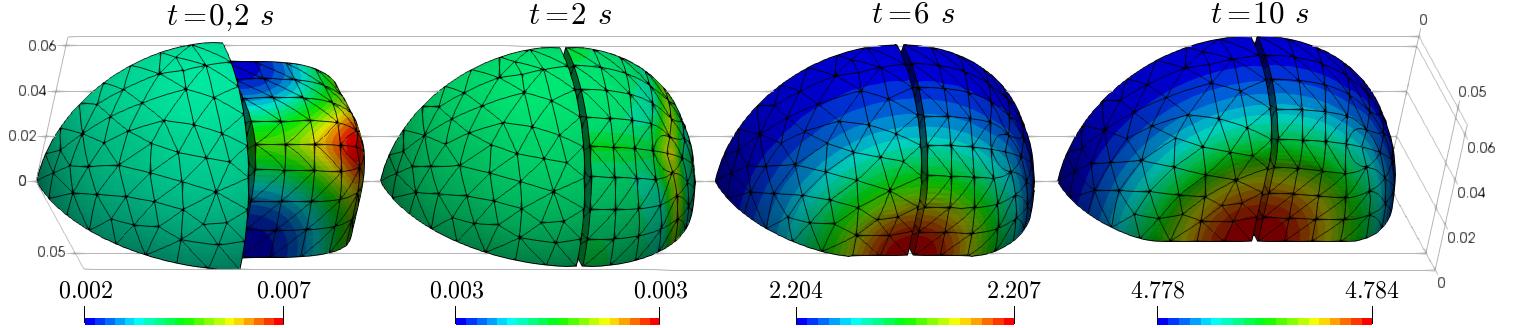
\includegraphics[width=\textwidth]{Figuras/PhaseChangeConsistencyTest3D/PTFE-a125e-4.png}
	%\caption*{\textbf{Fonte:} Elaborado pelo autor}
\end{figure}



\subsubsection{Derretimento de coluna: caso 2D}

Nesta seção, propomos uma generalização do problema apresentado na \cref{sec:barragem}, incorporando a mudança de fase. Neste caso, o domínio é inicialmente sólido e, através de um fluxo de calor aplicado em sua extremidade inferior, sua temperatura aumenta progressivamente, causando um derretimento gradual do material, que se propaga da base para o topo. 

Os dados do exemplo estão dispostos na \cref{fig:PhaseChangeDam}, incluindo geometria, condições de contorno, e parâmetros do material e da análise. As forças aplicadas incluem apenas o peso próprio e uma tensão superficial constante ao longo do tempo. Para a fase sólida, onde a rigidez é elevada, espera-se que essas forças provoquem apenas pequenas deformações. Assim, optamos por utilizar a lei de Saint Venant-Kirchhoff nessa fase, com estado plano de deformações (EPD).

\begin{figure}[!htb]
	\centering
	\caption{Dados do exemplo de derretimento de coluna 2D}
	\label{fig:PhaseChangeDam}
	{\small
		\noindent\shadowbox{
			\parbox{15.3cm}{
				\setlength{\columnseprule}{1pt}
				\vspace{-0.3cm}
				{\centering\begin{center}
						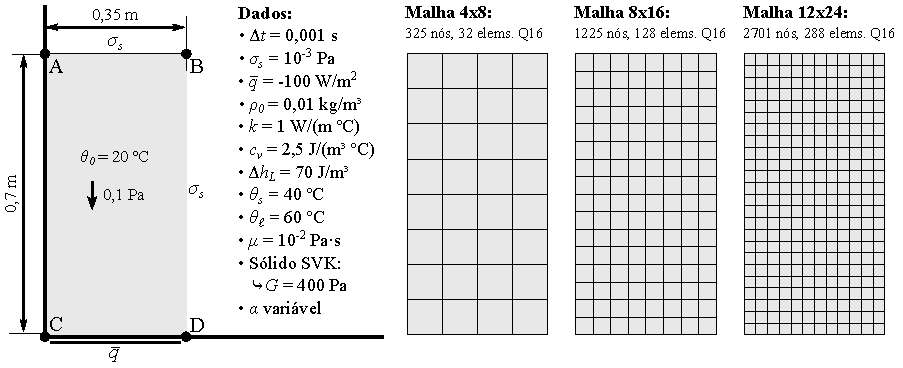
\includegraphics[scale=1.0]{Figuras/PhaseChangeDam/PhaseChangeDam.pdf}
					\end{center}\par}
				\vspace{-0.4cm}
			}
		}
	}	
	%\caption*{\textbf{Fonte:} Elaborado pelo autor}
\end{figure}


% !!!!!!!!!!! EM DESENVOLVIMENTO

Inicialmente, realizamos uma análise com o objetivo de verificar a sensibilidade dos resultados à discretização espacial, considerando as três malhas distintas da \cref{fig:PhaseChangeDam}. Nesta análise, não aplicamos expansão térmica, e utilizamos apenas o modelo com multiplicadores quínticos (\cref{tab:modelos}) para a fase de transição.

Na \cref{fig:PhaseChangeDamSolidToLiquid-meshConvergence}(a), é apresentado o gráfico de deslocamento horizontal no ponto D (canto inferior direito) ao longo do tempo. Como esperado, os deslocamentos são muito pequenos nos instantes iniciais (fase sólida), aumentando gradualmente à medida que o domínio passa pelas fases de transição e líquida. Podemos observar que esse gráfico apresenta resultados idênticos para as três malhas consideradas, ...

Além disso, na \cref{fig:PhaseChangeDamSolidToLiquid-meshConvergence}

, são apresentados os gráficos de deslocamento horizontal no ponto D (canto inferior direito), pressão no ponto C (canto inferior esquerdo), temperatura, e componentes líquida e sólida da deformação de Green-Lagrange no eixo horizontal.

Em seguida, utilizando apenas a malha 12x24, comparamos

é incorporada a expansão térmica exponencial com $\coefExp = 1\cdot 10^{-4}\,^{\circ}$C$^{-1}$, considerando apenas a malha 12x24. Em todos os casos, são comparados os três modelos de multiplicadores da \cref{tab:modelos} para a fase de transição.

\begin{figure}[!htb]
	\centering
	\caption{}
	\label{fig:PhaseChangeDamSolidToLiquid-meshConvergence}
	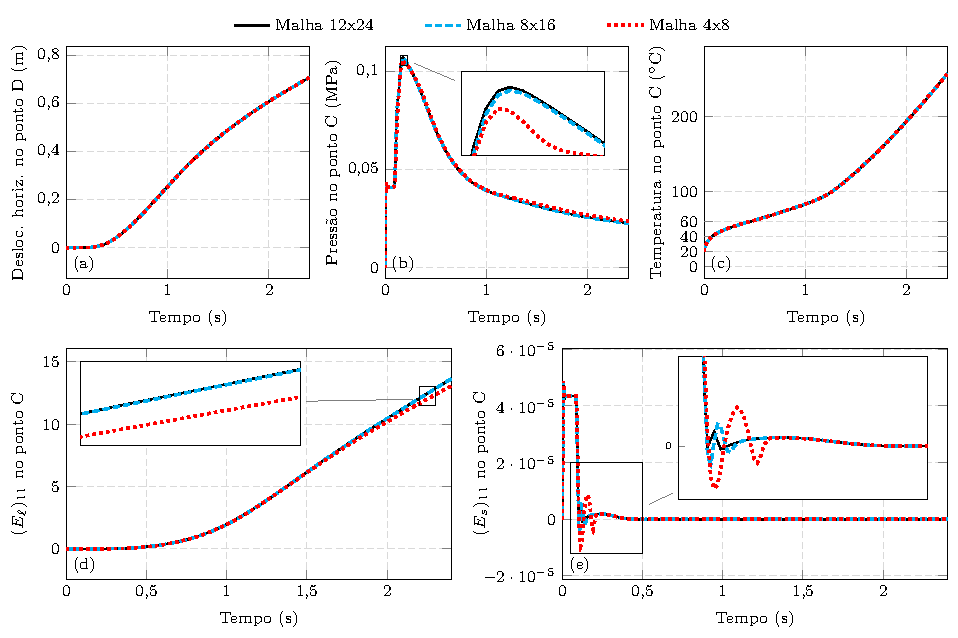
\includegraphics[scale=1.0]{Figuras/PhaseChangeDam/PhaseChangeDamSolidToLiquid-meshConvergence.pdf}
	%\caption*{\textbf{Fonte:} Elaborado pelo autor}
\end{figure}


 São ilustrados em mapas de cores as fases durante o processo (sólido, transição e líquido), as temperaturas, e as pressões.

\begin{figure}[!htb]
	\centering
	\caption{Configurações deformadas para o problema de derretimento de coluna com $\coefExp = 0$, e fases em mapa de cores}
	\label{fig:PhaseChangeDam-phase}
	\includegraphics[width=\textwidth]{Figuras/PhaseChangeDam/phase.png}
	%\caption*{\textbf{Fonte:} Elaborado pelo autor}
\end{figure}

\begin{figure}[!htb]
	\centering
	\caption{Configurações deformadas para o problema de derretimento de coluna com pressões (Pa) em mapa de cores, $\coefExp = 0$, multiplicadores quínticos e malha 12x24}
	\label{fig:PhaseChangeDam-pressure}
	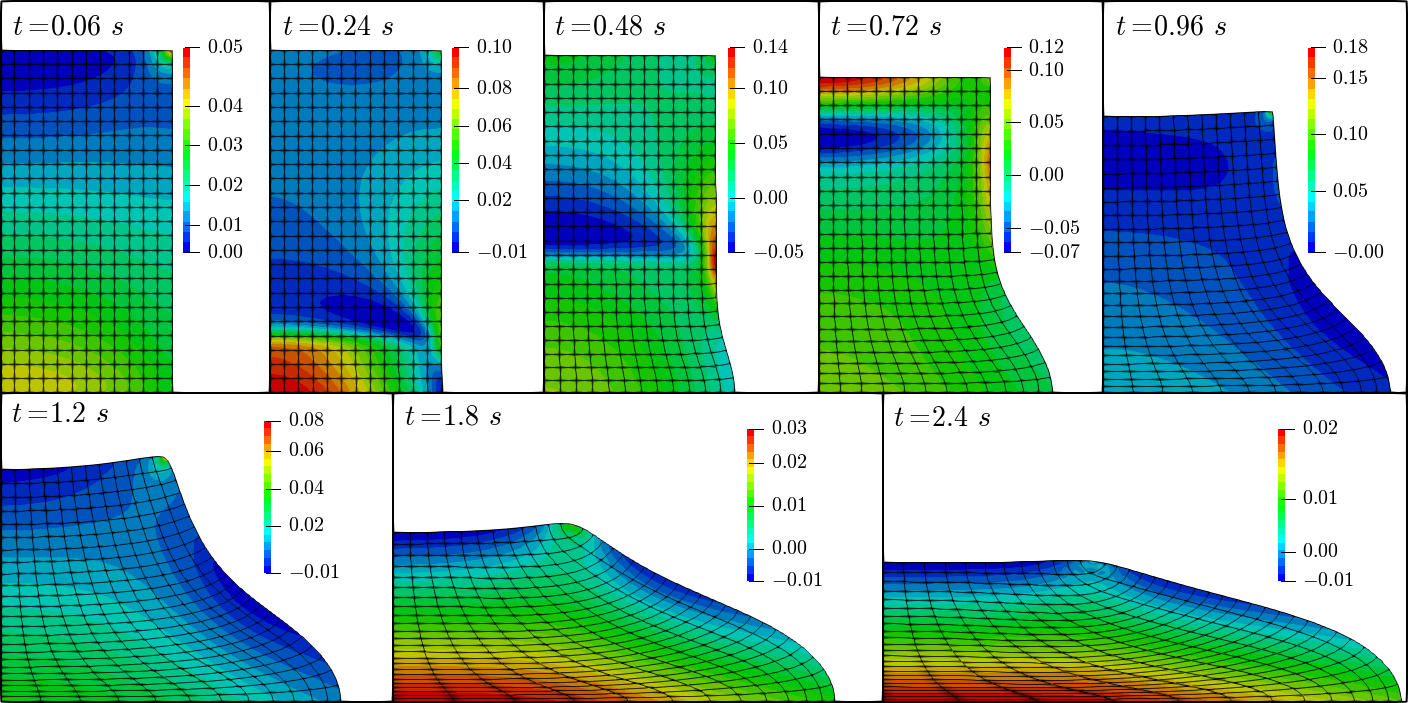
\includegraphics[width=\textwidth]{Figuras/PhaseChangeDam/pressure.png}
	%\caption*{\textbf{Fonte:} Elaborado pelo autor}
\end{figure}

\begin{figure}[!htb]
	\centering
	\caption{Configurações deformadas para o problema de derretimento de coluna com pressões (Pa) em mapa de cores, $\coefExp = 1\cdot 10^{-4}\,^{\circ}$C$^{-1}$, multiplicadores quínticos e malha 12x24}
	\label{fig:PhaseChangeDam-pressure-a1e-4}
	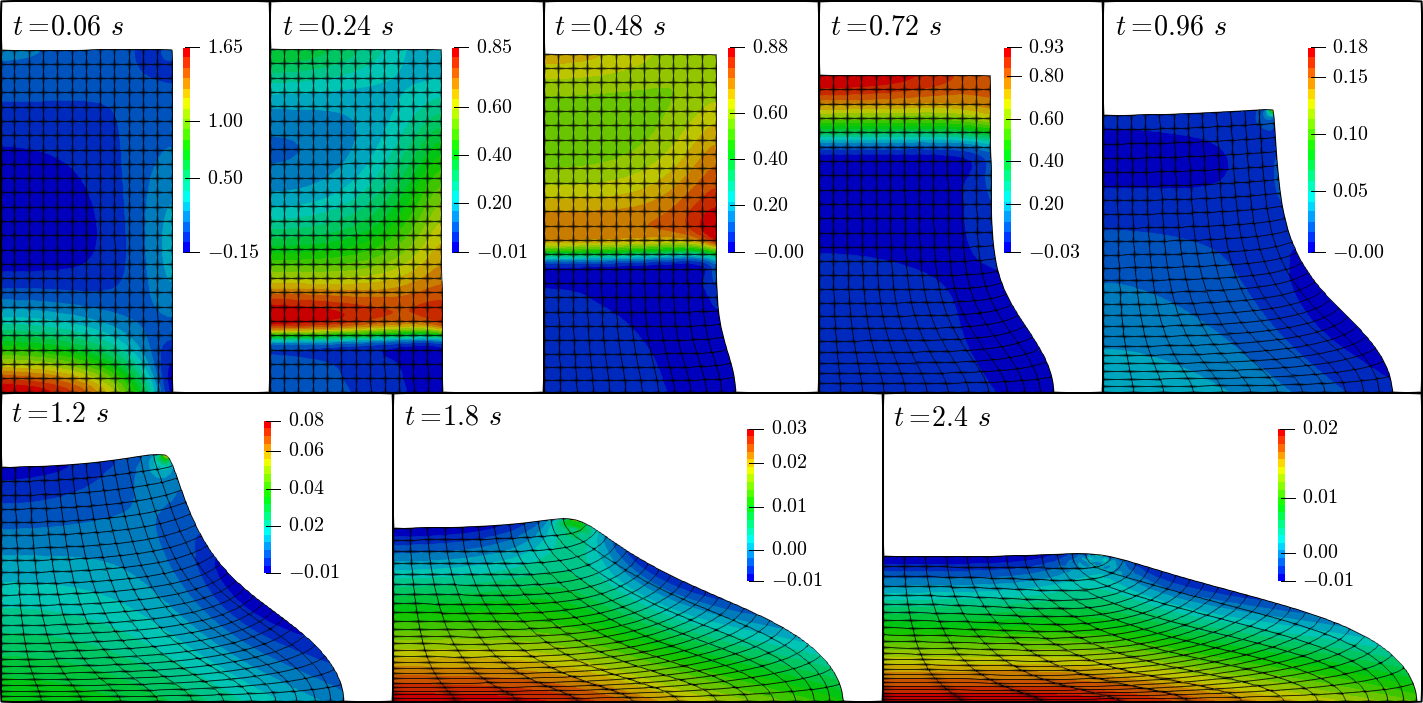
\includegraphics[width=\textwidth]{Figuras/PhaseChangeDam/pressure-a1e-4.png}
	%\caption*{\textbf{Fonte:} Elaborado pelo autor}
\end{figure}


\begin{figure}[!htb]
	\centering
	\caption{}
	\label{fig:PhaseChangeDamSolidToLiquid-multipliers-a0}
	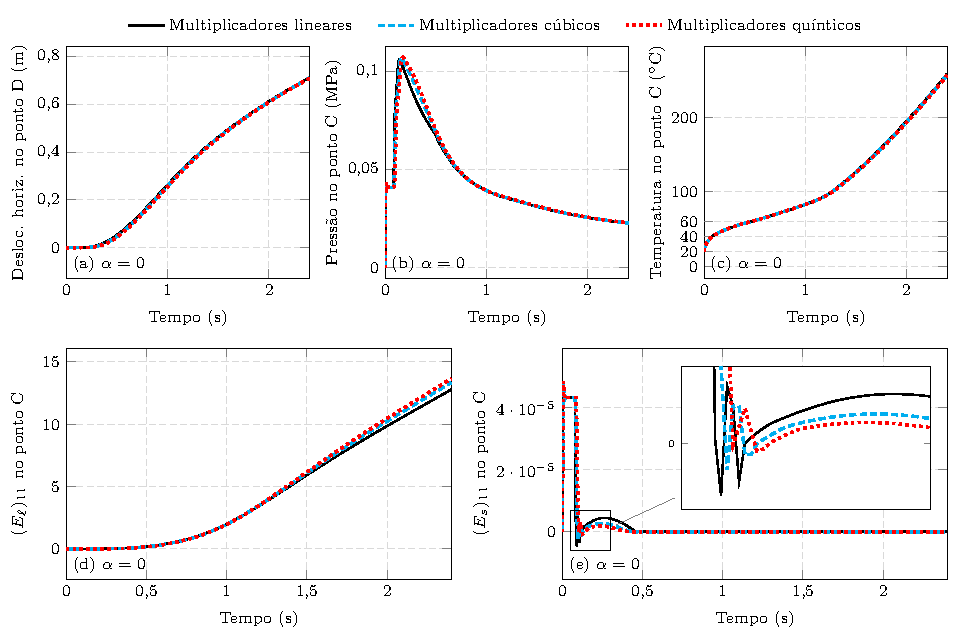
\includegraphics[scale=1.0]{Figuras/PhaseChangeDam/PhaseChangeDamSolidToLiquid-multipliers-a0.pdf}
	%\caption*{\textbf{Fonte:} Elaborado pelo autor}
\end{figure}

\subsubsection{Derretimento de coluna: caso 3D}

\begin{figure}[!htb]
	\centering
	\caption{Dados do exemplo de derretimento de coluna 3D}
	\label{fig:PhaseChangeDam3D}
	{\small
		\noindent\shadowbox{
			\parbox{15.3cm}{
				\setlength{\columnseprule}{1pt}
				\vspace{-0.2cm}
				{\centering\begin{center}
						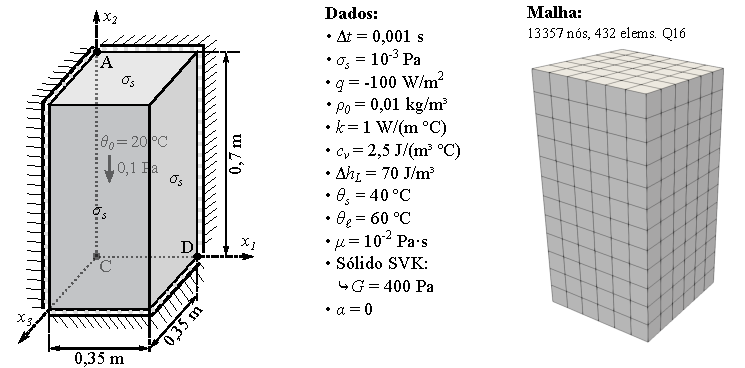
\includegraphics[scale=1.1]{Figuras/PhaseChangeDam3D/PhaseChangeDam3D.pdf}
					\end{center}\par}
				\vspace{-0.3cm}
			}
		}
	}	
	%\caption*{\textbf{Fonte:} Elaborado pelo autor}
\end{figure}

\begin{figure}[!htb]
	\centering
	\caption{Configurações deformadas para o problema de derretimento de coluna 3D com multiplicadores quínticos, e fases em mapa de cores}
	\label{fig:PhaseChangeDam3D-phase}
	\includegraphics[width=\textwidth]{Figuras/PhaseChangeDam3D/phase.png}
	%\caption*{\textbf{Fonte:} Elaborado pelo autor}
\end{figure}

\begin{figure}[!htb]
	\centering
	\caption{Configurações deformadas para o problema de derretimento de coluna 3D com multiplicadores quínticos, e pressão (Pa) em mapa de cores}
	\label{fig:PhaseChangeDam3D-pressure}
	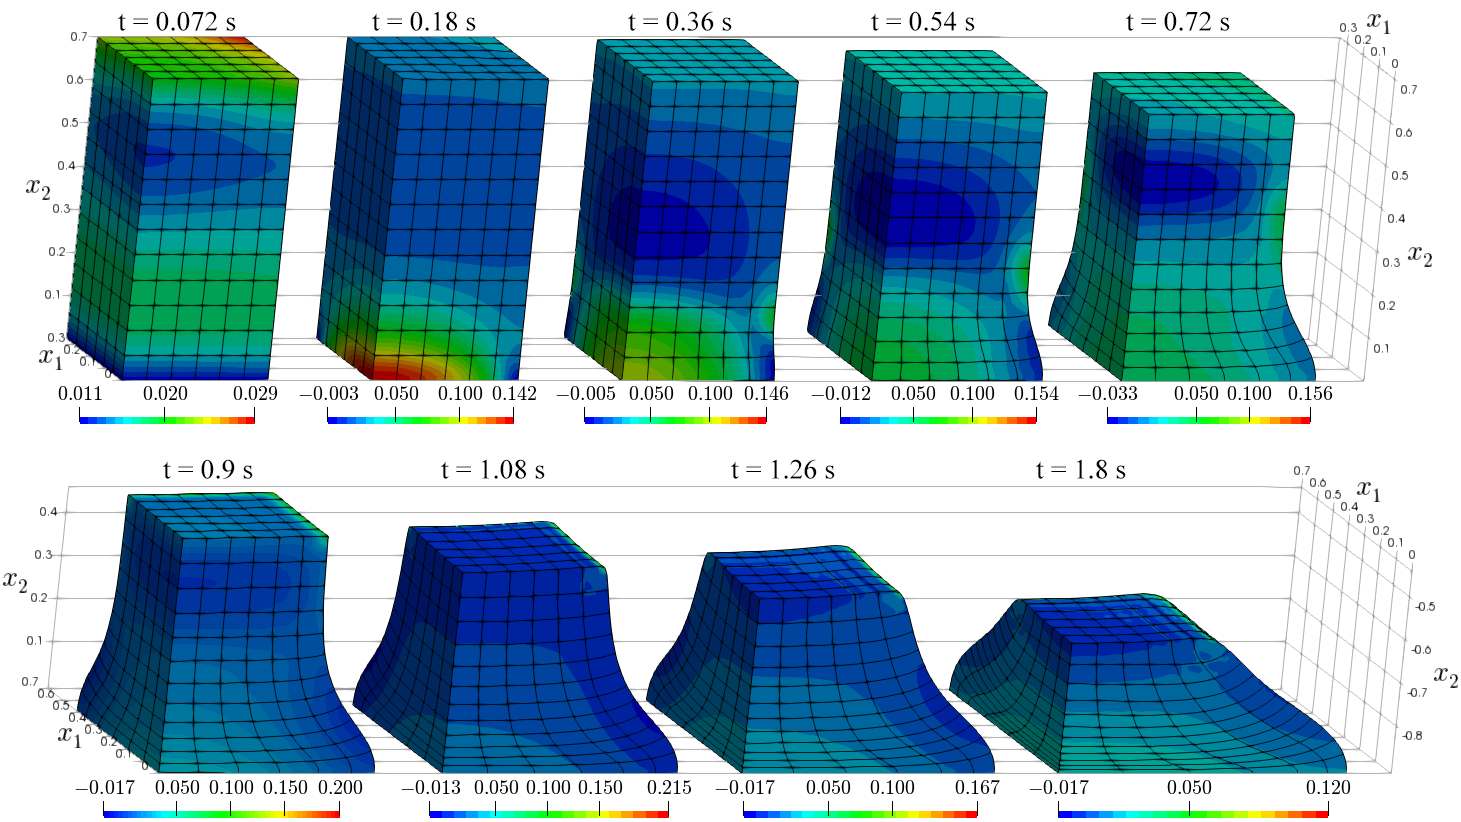
\includegraphics[width=\textwidth]{Figuras/PhaseChangeDam3D/pressure.png}
	%\caption*{\textbf{Fonte:} Elaborado pelo autor}
\end{figure}

\begin{figure}[!htb]
	\centering
	\caption{}
	\label{fig:PhaseChangeDamSolidToLiquid3D-multipliers}
	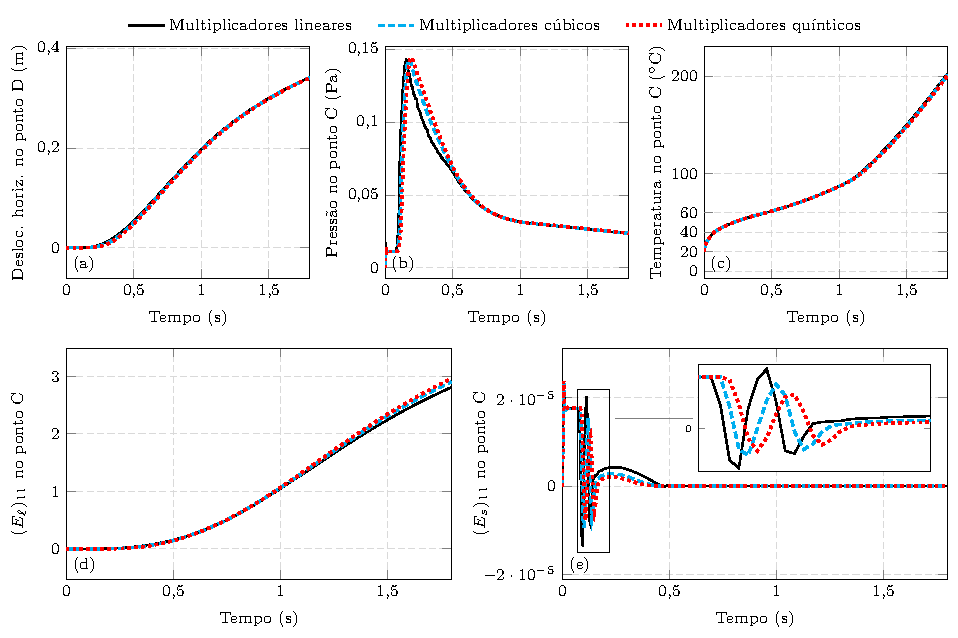
\includegraphics[scale=1.0]{Figuras/PhaseChangeDam3D/multipliers.pdf}
	%\caption*{\textbf{Fonte:} Elaborado pelo autor}
\end{figure}

\end{document}